\documentclass[]{kththesis}
\usepackage{csquotes} % Recommended by biblatex
\usepackage[style=numeric,sorting=none,backend=biber]{biblatex}
\usepackage[swedish]{babel}
\usepackage[]{graphicx}

\graphicspath{{../images/}}

\addbibresource{references.bib}

\title{Find objects in real estate images with convolutional neural networks}
\alttitle{Hitta object i fastighetsbilder med convolutional neural networks}
\author{Oskar Råhlén och Sacharias Sjöqvist}
\email{orahlen@kth.se och sacsjo@kth.se}
\supervisor{Handledare}
\examiner{Examinator}
\programme{Degree project in Computer Science}
\school{School of Electrical Engineering and Computer Science}
\date{\today}

% Uncomment the next line to include cover generated at https://intra.kth.se/kth-cover?l=en
% \kthcover{kth-cover.pdf}

\begin{document}
\frontmatter

\begin{abstract}
    English abstract goes here
\end{abstract}

\begin{otherlanguage}{swedish}
  \begin{abstract}
    Svenskt sammanfattning
  \end{abstract}
\end{otherlanguage}
  
\tableofcontents

\mainmatter
% Citera med \texttt{} och \parencite{}

\chapter{Introduktion}
Koppla första mening till titel. söka på speicfika saker i en annons. mysig inledning. Deeplearning bildanalys - google grejer. Ai och hur automatisering vuxit fram. Lite fakta på hur viktig sökfunktioner är för att hitta bostäder? Hur många sökningar /tidsenehet. Om folk enklare hittar bostad på ett mer effektivt sätt så effektiviseras hela köp och sälj processen och därmed hela marknaden.

Just nu (april 2019) finns över 20 000 bostadsrätter (https://www.hemnet.se/statistik) till salu på Sveriges största mäklarsite (https://www.hemnet.se/om), där nästan hälften av dessa ligger i Stockholm. 
Dit kommer 2,8 miljoner (https://www.hemnet.se/om) unika besökare varje vecka och gör tillsammans över 2000 sökningar i minuten.
Detta ställer höga krav på filtreringsfunktionerna för att potentiella köpare snabbt ska kunna hitta sin drömbostad.
Idag erbjuds redan filtreringsfunktionerna ”antal rum”, ”boarea”, ”pris” samt ”område”. 
Det finns också en fritextsöka där man kan söka på vad mäklaren har skrivit i texten.
Exempel på sökord är ”balkong”, ”kakelugn” och ”sjöutsikt”. 

Problemet med att söka i mäklartexter är att det tvingar mäklaren att i texten nämna samtliga attribut som han eller hon vill göra sökbara. 
Detta gör att vissa attribut kan bli utelämnade vilket i sin tur gör fritextrutan sämre.

Exempelvis är det ofta självklart om det finns en balkong eller kakelugn på mäklarbilderna men det är inte alltid mäklaren väljer att skriva detta i den löpande texten.
Det hade därför varit intressant att utifrån mäklarbilderna automatiskt generera ett sökindex där varje bild knyts till ett antal attribut.
Dessa attribut skulle sedan kunna användas för att lägga till filtreringsalternativ i sökfunktionen och därmed skapa en bättre användarupplevelse.

Det skulle också gå att använda sig av denna metod för att knyta attribut såsom skick och typ av rum (Sovrum, badrum eller kök) till varje bild.
Kombinationen skulle göra sökningar såsom ”Kök i gott skick” möjligt.  

Denna data kan också vara användbar vid värdering av bostäder, då det enkelt skulle gå att jämföra priser på bostäder med olika attribut, tillexempel lägenheter med sköutsikt mot lägenheter utan sköutsikt eller lägenheter med ett kök i gott skick mot lägenheter med ett kök i sämre skick.

VET INTE RIKTIGT HUR JAG SKA FORMULERA MIG HÄR!! Känns Som ett halvbra stycke
För att på ett effektivt och precist sätt kunna knyta attribut till mäklarbilder behöver man använda sig av någon form av automatisk bildbehandling.
Detta går att göra med hjälp av maskininlärning och djupa neurala nätverk.
Sättet som detta görs på är att man tränar ett antal bilder som innehåller det givna attributet och ett antal som inte innehåller attributet.
Modellen tränas sedan med hjälpt av ett djupt neuralt nätverk. 
Efter varje träning så testas modellen för att mäta hur många träningar som krävs för bästa resultat.
När modellen är färdigtränad kan man använda denna genom att skicka in en bild som input och modellen berättar om bilden innhåller attributet eller inte.
 



\section{Syfte}
Syftet med denna studie är att titta på hur olika maskininlärningsmetoder kan användas för att hitta relevanta nyckelord till bilder på lägenhetsannonser. 

\section{Frågeställning}
Går det med nuvarande verktyg inom maskininlärning hitta attribut i bilder från lägenhetsannonser?

\section{Avgränsningar}
För att sätta en rimlig avgränsningar på denna uppsats kommer tre olika sorters attribut undersökas och jämföras med tre olika sorters deeplearningmodeller. 
Attributen som kommer– användas är ”Balkong”, ”Kakelugn” samt ”Typ av rum” (Kök, badrum eller sovrum) och deelearningmodellerna som kommer användas är ”keras”, ”smartAI”, samt ”blabla”. 
Anledningen till att flera attribut eller flera sorters modeller inte valdes är att det är resurskrävande att både samla in och sortera testdata samt att implementera modellerna. 
Anledningen till att färre inte valdes var för att få spridning på attributen och modellerna, för kunna svara på om klassifiseringen fungerar i allmänhet och inte bara i enstaka testfall. 
En annan avgräsning som gjort är att mäklarbilderna som används endast kommer från bostadsrätter, då det kan skilja sig ganska mycket på hur villor och bostadsrätter ser ut.

\chapter{Bakgrund}
I det här kapitlet presenteras teori som är relevant för bildklassificering. Målet är att ge läsaren förståelse för de byggstenar som används för att konstruera en modern algoritm för bildklassificering. De vanligaste verktygen inom modern bildkategorisering bygger på djupinlärning, som är en del inom
artificella neurala nätverk.

\section{Maskininlärning}
Maskininlärning är ett aktivt forskningsfält inom datalogi och en maskininlärningsalgoritm kan förklaras som en algoritm som lär sig att bli bättre med hjälp utav data \parencite{Goodfellow-et-al-2016}. Inom maskininlärning så brukar lärandeprocessen se ut på följande sätt: Om ett datorprogam har som uppgift att med hjälp av en viss erfarenhet E, lära sig vissa förutbestämda uppgifter T, vilket kan mätas med måttet P. Om programmets prestanda P blir bättre, det vill säga att programmet blir bättre på att lösa uppgifterna T, med hjälp av erfarenheten E, då lär sig programmet.

Maskininlärning brukar delas in i två överkategorier: Unsupervised learning och Supervised learning. Det som skiljer dessa åt är att inom supervised learning så är all data redan kategoriserad och uppmärkt för ändamålet medan inom unsupervised learning så är den inte det. Det kan ses som att vi i ena fallet redan har de rätta svaren på vår data. Algoritmer inom unsupervised learning handlar huvudsakligen om att kategorisera data i olika kluster eller på andra sätt försöka förstå den tillgänliga datan. Supervised learning handlar istället om att utgå ifrån den uppmärkta datan och lära sig utav den för att göra samma typ av kategorisering som datan redan är kategoriserad i. Denna funktionsapproximation kan sedan användas för klassificering av ny omärkt data. Det finns även andra grenar tillämpningsområden inom supervised learning utöver klassificering.

\section{Artificella Neurala Nätverk}
Ett område med många tillämpningsområden inom maskininlärning är artificella neurala nätverk. Neurala nätverk var från början ett försök till att bygga en digital modell av hur det biologiska neuronsystem fungerar. Forskningen inom områden avvek sedan från att efterlikna den biologiska varianten så mycket som möjligt och fokuserade istället på att konstruera neurala nätverk som fungerade så bra som möjligt på maskininlärningsproblem. Grundbyggstenarna i neurala nätverk är dock fortfarande baserade på dess biologiska variant. Den enklaste beräkningsenheten i hjärnan är en neuron och dessa neuroner är ihopkopplade med synapser. En neuron får signal in och skickar sedan signaler ut via synapserna. Hur stark utsignal är simuleras i en dator med hjälp av vikter, (engelska: weights, W). Målet är att träna modellen och göra den bättre genom att justera vikterna. Om summan av flera av dessa viktade insignaler når en viss gräns, så skickar neuronerna vidare en signal. Detta simuleras i en dator med en aktiveringsfunktion. Neurala nätverk är dessa neuroner i en acyklisk graf.
  

[BILD PÅ NEURALT NÄTVERK]

Ett vanligt neuralt nätverk består vanligtvis först av ett indatalager (input layer). Indatalagret brukar representeras av en neuron per egenskap i indatan. Då indata är bilder så brukar en neuron i indatalagret motsvara en pixel i en bild. Dessa neuroner i indatalagret är sedan ihopkopplade med ett nytt lager med neuroner. Detta lager kallas för det gömda lagret (hidden layer). De gömda lagren kan bestå av godtyckligt många neuroner. Det går att ha en eller fler gömda lager efter varandra och efter det kommer utdatalagret (output layer). Utdatalagret består vanligtvis av lika många neuroner som modellen ska ge olika svar. Om modellen ska kategorisera indata i tio olika kategorier, så borde modellen då ha tio neuroner i sitt utdatalager.

Ett neuralt nätverk blir bättre på sin uppgift genom att ändra sina vikter, vilka även kallas för parametrar. Detta sker i två steg. Första steget är feed-forward pass. Feed-forward pass handlar om att skicka in sin träningsdata genom nätverket och få ut ett svar eller klassificering. Då träningsdatan redan är uppmärkt så jämfört svaret från det neurala nätverket med det riktiga svaret. Beroende på hur många fel nätverket gissade och hur osäker det var när det gissade fel, så beräknas en kostnad. Det finns olika sätt att beräkna denna kostnad men vanligtvis används cross-entropy loss. Målet med att träna modellen är att få denna kostnad så låg som möjligt. Nästa steg är backward pass, vilket även kallas för backpropagation. Det vi vill göra är att ändra parametrarna så att kostnaden vi beräknade innan blir lägre. Detta görs genom att beräkna gradienten av kostnaden med avseende på alla parametrarna. Vi kan sedan ta ett steg åt motsatt håll som gradienten, för att minska kostnaden. Storleken på detta steg kallas för learning rate.

\subsubsection{Stochastic gradient descent}
Stochastic Gradient Descent heter den vanligaste algoritmen för att uppdatera parametrarna med hjälp av gradienten. Den bygger på samma tvåstegsmodell som beskriven ovan men istället för att beräkna gradienten för alla datapunkter i träningsmängden så väljs några stycken ut som man beräknar gradienten på. Denna delmängd brukar kallas för batch och dess storlek för batch size. En epoch är när modellen har gått igenom alla datapunker i träningsmängden en gång. Learning rate är då hur stort steg åt gradientens motsatta håll vi ändrar på parametrarna vid varje uppdatering.

[FORMEL PÅ SGD]

En förbättring till learning rate är the momentum method. Stochastic gradient descent med momentum kommer ihåg förändringen av parametrarna vid varje iteration och baserar nästa uppdatering på en linjärkombination av gradienten och den tidigare förändringen. 

[FORMEL PÅ MOMENTUM]

\section{Convolutional Neural Network}
Convolutional neural networks (CNN) är en viss typ av neurala nätverk för att processera data som har indata som är placerat i ett rutnät. Det inkluderar data om tidsserier men även bilddata, som kan ses som ett rutnät av pixlar. CNN har fått stort genomslagskraft i praktiska tillämpningar. Convolution är en viss typ av linjär operation och CNN är då neurala nätverk där minst ett av dess lager är ett convolutional layer.

CNN har blivit den dominanta approachen inom maskininlärning för igenkänning av visuella objekt \parencite{huang2017densely}. Även om CNN introducerades för 20 år sedan, så har förbättringar i hårdvara och nätverksstruktur gjort det nyss möjligt att träna djupa CNN \parencite{huang2017densely}.



\subsection{Lager}
Här presenteras de lager som vanligtvis används i ett CNN. Detta för att sedan kunna gå in på hur de olika arktitekterna inom CNN är uppbyggda. Även om CNN kan användas till olika typer av data, så fokuserar vi här i texten på dess kontext med bilder. En vanlig ordningsföljd av lager för bildkategorisering är input, convolutional layer, ReLU, pooling layer och sist ett fully-connected layer.

\subsubsection{Input}
Detta lager håller de råa pixelvärdena från bilden via skickar in. I ett vanligt neuralt nätverk med resnet-arkitekturen så är det 224 x 224 x 3. Då är det en rektangulär bild med 224 pixlar i höjd, 224 pixlar i bred och 3 färgkanaler, RGB.

\subsubsection{Convolutional Layer}
Ett convolutional layer består av en mängd filter som har parametrar som går att träna. Varje filter är kvadratiskt och små mått i höjd och bredd, men har alltid samma djup som vår indata. En vanlig storlek på ett filter är 5x5x3, det vill säga 5 pixlar brett och högt och 3 färgkanaler. Vid forward pass så glider vi (convolve) detta filter över vår indata-bild. Vi beräknar skalärprodukten av filtret och den 5x5x3-bit av indatan som filter ligger på. Efter beräkningen så glider vi filtret åt sidan. Vanligtvis en pixel, men det kan även vara flera. Utdata från varje filter blir en tvådimensionell activation map. Djupet på utdata motsvarar antal filter vi använt i vårt convolutional layer. Höjd och bredd på utdata beror på storleken på filter.

Storleken på utdata från ett convolutional layer beror på tre hyperparametrar: djup, stride och zero-padding. Djup motsvarar antal filter som används och blir djupet på vår utdata. Stride består hur många pixlar vi förflyttar oss vid varje glidning. Zero-padding bestämmer om vi ska bygga en ram runt bilden med nollor. Detta användas för att kunna behålla storleken på bilden igenom flera convolutional layers men är också bra för att inte bortse viktig information i utkanten av bilden.

\subsubsection{Activation Layer / ReLU}
Activation Layer består av en elementvis funktion. Det finns flera olika typer av dessa, men det som vanligtvis används inom bildkategorisering är Rectified Linear Units (ReLU). Den applicerar funktionen max(0,x) på varje element i indata. Detta betyder varje element som är positivt är opåverkat och varje negativt värde får värdet noll. Utdata har samma storlek som indata.

\subsubsection{Pooling Layer}
Ett pooling layer applicerar en nedsampling (eng: downsampling) på indata. Detta sker längs de spatiala dimensionerna, bredd och höjd. Detta sker vanligtvis för att minska antalet parametrar i nätverket och för att minska på beräkningskraften som behövs. Det är även en teknik för att undvika overfitting. Vanligaste typen är max pooling, då man tar ett område, till exempel 2x2 pixlar och väljer den pixel med högst värde. Vanligast är max pooling på 2x2 pixlars filter med en stride på 2. Indata minskar då med 75\%.

\subsubsection{Fully-connected Layer}
Fully-connected layers är den typen av lager som är vanligast i normala neurala nätverk. I detta lager har varje neuron en full koppling till alla aktiveringar från det tidigare lagret. Dessa har då vanligtvis en tillhörande matris med vikter och bias, vilket kan beräknas med matrismultiplikation. Storleken på utdata beror på storleken på viktmatrisen. Vanligtvis så byggs det sista FC layer upp så att det har samma storlek som vi vill ha kategorier. Om vi vill klassifiera en bild i tio kategorier, så kan utdata från vårt sista lager ha storleken 10x1, där varje element motsvarar sannolikheten för att bilden tillhör en viss kategori.

\subsection{Tekniker inom djupinlärning}

\subsubsection{Batch normalization}

\subsubsection{Data augmentation}

\subsection{Arkitekturer}
Här kommer ett urval av de vanligaste arkitekturerna för CNN för bildkategorisering att presenteras. Nätverk med conv-lager har blivit djupare och djupare, från LeNet \parencite{lecun1998gradient} med fem lager, VGG med 19 lager \parencite{simonyan2014very} och Residual Networks (ResNet) med över 100 lager \parencite{he2016deep}. Ett problem med detta är att viktig information i indata försvinner innan det hinner nå slutet av nätverket \parencite{huang2017densely}. Det har därför kommit arkitekturen som försöker lösa dessa problem. ResNet löser det genom att förbikoppla vissa lager med identitetskopplingar. DenseNet skapar flera olika förbikopplingar inne i nätverket.

\subsubsection{Resnet}
Det finns flera olika varianter av ResNet, Resnet18, Resnet34, Resnet50, Resnet101 och Resnet152, beroende på storlek. Vi fokuserar här på Resnet18. ResNet bygger på en struktur med convolutional layers, pooling layers och fully-connected layers. Trenden har varit att CNN blir djupare med fler lager.

Men till slut kom modellerna till ett tak när det handlar om accuracy. ResNet är en lösning på det här problemet genom att introducera "identity shortcut connections". Detta betyder att det finns kopplingar som hoppar över vissa convolutional layers. Det betyder att om modellen inte behöver utnyttja alla convolutional layers så kan den bara använda sig av identiteten istället för ett convolutional layer. Det betyder att nätverket borde kunna vara hur stort som helst, för det går alltid att bara använda indentiteten. Modellerna med residuala funktioner ska även vara enklare att optimera \parencite{he2016deep}. Resnet beskär bilderna till storleken 224 x 224 pixlar, och huvudsakliga målet var att kategorisera bland 1000 kategorier i imageNet 2012 classification dataset. Det finns flera olika versioner av ResNet, beroende på antal lager. ResNet-18 består totalt av 18 lager, när det första lagret är ett convolutional layer och därefter ett max pooling-lager. Därefter är det många convolutional layer där det även sker en nedsampling. Till sist är det ett average pooling-lager, ett fully connected-layer med output 1x1000 och ett softmax-lager, som gör att de olika outputvärdena kan ses som en distribution. 

\subsubsection{Alexnet}
Alexnet är en enklare variant av CNN och består av totalt åtta lager \parencite{krizhevsky2012imagenet}. De första fem lagrena är convolutional layers, där vissa av dem har max pooling-lager emellan sig. De tre sista är fully connected-layers, där det sista har output 1x1000 för att motsvara klasserna i imagenet. Det sista lagret är också softmax. Alexnet använder sig av aktiveringsfunktionen ReLU. AlexNet vann ILSVRC 2012. Indata har storleken 224x244. De olika lagrena består av 11x11, 5x5, 3x3, convolutions, max pooling och ReLU aktiveringsfunktioner. Det tränades ursprungligen med SGD med momentum.

\subsubsection{VGGNet}
Enligt \cite{simonyan2014very} så har VGG högre noggrannhet än Alexnet och uppnådde år 2015 state-of-the-art noggrannhet på ILSVRCs klassificering och lokaliseringsuppgifter. Alla conv-lager följer samma design som den i Alexnet \parencite{simonyan2014very}. 

Enligt \cite{simonyan2014very} ser arkitekturen ut som följande: Under träning så består indata av RGB-bilder av fixerad storlek 224 x 224. Den enda förbehandlingen är att medelvärdet av RGB-värdena som beräknas på träningsmängden subtraheras från varje pixel. Bilden skickas sedan igenom en stack av conv-lager med filter av storlek 3 x 3. I en av konfigurationerna används även 1 x 1-filter, som kan ses som en linjär transformation av indatakanalerna. Kliven, Stride, är 1 pixel och padding beror på filterstorlek, men ska se till att indata och utdata är i samma storlek. Padding är 1 pixel vid 3 x 3-filter. Spatial pooling sker med fem stycken max-pooling lager, där vissa följer efter conv-lager. Det är inte alla conv-lager som följs av max-pooling. Max-pooling sker med ett 2 x 2-filter med stride 2. En stack av conv-lager, som är olika djup beroende på vilken typ av VGG, följs sedan av tre stycken FC-lager. De första två har 4096 kanaler var och det sista har 1000-kanaler, för att motsvara klasserna i ILSVRC-problemet. Det sista lagret är ett soft-max-lager. Alla gömda lager är utrustade med ReLU icke-linjäritet. 

\subsubsection{Densenet}
Tidigare forskning har visat att nätverk bestående av conv-lager kan vara djupare, har högre noggrannhet och är mer effektiva att träna om det finns kortare vägar mellan indata och utdata \parencite{huang2017densely}. Därför skapades DenseNet, vilket kopplar ihop varje lager i nätverk med varje lager framför. Det betyder att om ett tradionellt nätverk med conv-lager har totalt L antal lager, så har det även L kopplingar. DenseNet har istället L(L+1)/2 antal direkta kopplingar. Enligt \cite{huang2017densely} så har DenseNet uppnått signifikanta förbättringar på Cifar-10 och ImageNet jämfört med andra state-of-the-art-modeller. Det betyder att alla lager har en direkt koppling till alla lager framför. DenseNet har olika intern arkitektur beroende på storlek. Gemensamt är dock att indata består av RGB-bilder av storlek 224 x 224. Därefter kommer en stack med conv-lager där första lagret har filterstorlek 7 x 7 och stride 2. Efterkommande conv-lager kommer i par, där det första i paret har storlek 1 x 1 och den andra har filterstorlek 3 x 3. Stride 1 och padding för att behålla storleken på indata. Mellan dessa lager sker först max-pooling med storlek 3 x 3 och stride 2 och sedan average pooling med storlek 2 x 2 och stride 2. Sista lagret, som är klassificeringslagret, består av global average pooling med storlek 7 x 7 och ett FC-lager med 1000 kanaler som ett soft-max-lager.

\subsubsection{Inception-v2}
Inception har en mycket lägre beräkningskostnad än VGG \parencite{szegedy2016rethinking}. Detta har lett till att den används i big-data-sammanhang, där modeller med större beräkningskraft inte har kunnat användas. Inception-v2 består av en stack med conv-lager där alla har filterstorlek 3 x 3 med stride 1 eller 2. Det finns även mellan conv-lagren ett max pooling med storlek 3 x 3 och stride 2. Padding är så data ska behålla storleken. Därefter kommer tre stycken inception-lager. Ett inception-lager är ett lager som kombinerar resultatet från flera olika conv-lager i olika storlekar (vanligtvis 1 x 1, 3 x 3 och 5 x 5) ihop med ett max pooling-lager. Efter inception-lagren kommer klassificeringslagren som består av ett max pooling med storlek 8 x 8, ett FC-lager med 2048 kanaler och sist ett FC-lager med 1000 kanaler med softmax.

Inception-v2 är unikt då det består av två utdatalager vid träning. \parencite{szegedy2016rethinking} Det primära lagret är ett linjärt lager i slutet av nätverk medan det sekundära lagret kallas för auxiliary output. Vid testning så används bara det primära lagret.

\section{Transfer Learning}
Enligt \cite{yosinski2014transferable} så har många djupa neurala nätverk som har tränats på naturliga bilder visar att de har en gemensam sak. Det är att i de första lagren så lär de sig egenskaper som motsvarar Gabor-filter och färgklickar. Gabor-filter är ett typ av filter som används för att beskriva textur. 


\subsection{ImageNet}

\subsection{Feature extraction}

\subsection{Finetuning}

\chapter{Metod}
Detta kapitel kommer att beskriva metoden som användes för att ge mäklarbilder attribut.


\section{Datainsamling}
För att kunna träna modeller för de olika attributen ”balkong”, ”kakelugn” samt ”typ av rum” behövdes ett antal bilder som både uppfyllde dessa attribut samt ”negativa” bilder som inte uppfyllde dessa attribut.
Detta gjordes med ett pythonscript som heter Google Images Download (https://github.com/hardikvasa/google-images-download) och tar ett sökord, hur många bilder som ska laddas ner (X) samt från vilken källa bilderna ska hämtas från som input och ger tillbaka en mapp med de första X antal bilderna som hittas på Google från den givna källan. 

Bildkällan som valdes var https://hemnet.se då det är Sveriges största bostadsförmedlingssite med mängder av bilder.

Sökorden samt antalen som användes för detta beskrivs här:

\begin{center}
  \begin{tabular}{ |c|c|c| } 
   \hline
   Sökord & Antal \\ 
   \hline
   balkong hemnet & 400  \\ 
   \hline
   balkong vasastan & 400 \\ 
   \hline
   balkong inspiration & 400 \\ 
   \hline
   hemnet vardagsrum & 400  \\ 
   \hline
   hemnet badrum & 400 \\ 
   \hline
   Hemnet braskamin & 400  \\ 
   \hline
   hemnet öppen spis & 400 \\ 
   \hline
   vardagsrum braskamin & 400 \\ 
   \hline
   hemnet hall & 400 \\ 
   \hline
   hemnet kök & 400 \\ 
   \hline
   hemnet uteplats & 400   \\ 
   \hline 
  \end{tabular}
  \end{center}

Eftersom denna data inte är validerade mäklarbilder med det attribut som sökes påbörjades ett valideringsarbete där alla bilder manuellt validerades och sorterades enligt följande:
\begin{itemize}
  \item Alla bilder som inte uppfattades som mäklarbilder enligt definitionen ovan raderades
  \item Alla bilder som inte var tagna på lägenheter raderades
  \item Alla bilder med en eldstad las i en mapp med eldstäder
  \item Alla bilder med en balkong las i en mapp
  \item Alla bilder på ett kök las i en mapp
  \item Alla bilder på ett vardagsrum las i en mapp
  \item Alla bilder på ett badrum las i en mapp
  \item Negativa bilder skapades för samtliga mappar. Alltså skapades en mapp med bilder utan eldstad, en mapp med bilder utan balkong etc. Dessa skapades med hjälp av bilder i övriga mappar. 
\end{itemize} 

I varje mapp låg det slutligen runt 400 bilder. 

När detta var slutfört delades varje mapp i ytterligare två delar, en som kallades ”training” och en som kallades ”validation”.
I training palcerades de första 80\% av bilderna och i validation de sista 20\%.
Detta gjordes för att kunna testa hur modellerna presterade när de var färdigtränade med 20\% av den totala bildmassan.


\section{Modeller}
För att träna modellerna användes Python 3.6 med deeplearningramverket Pytorch 1.0.0. 
Modellerna tränades med  hjälp av pytorch i de olika ramverken ”Resnet”, ”Alexnet”, ”VGG-11”, ”Densenet” samt ”inception V3”.
Efter varje träningsrund (Epoch) kördes en validering för att se hur förbättringskurvan ser ut efter varje Epoch och när modellen börjar bli ”overfitted”.

Dessa modeller kördes ett antal epochs? och bla bla bla bla

\section{Uppföljning}
När modellerna var färdigtränade gjordes ett utdrag av statistik för att kunna jämföra modellerna sinsemellan.
Datan som hämtades för varje modell var


\section{Hårdvara}
Hårdvaran som användes när modellerna tränades var följande:

\subsection{Graphical processing unit (GPU)}
GPUn som användes var av modell Tesla K80 och hade tillgång till 128GB grafikminne.

\subsection{Central processing unit (CPU)}
CPUn som användes hade fyra kärnor 

\subsection{Random Access Memory (RAM)}
Det fanns tillgång till 61GB RAM-minne.


Hur vi gått tillväga. Vilka dataset, hur implementation gått till (verktyg, klassificerare, parametrar), hur vi valt features.
Hur evalueringen har gått till (traning, test, validation set).
\chapter{Resultat}
Prestandan av de olika modeller kommer presenteras här.

\section{Balkonger}
Här nedan presenteras resultatet av den binära klassificeringen av balkonger i mäklarbilder. Resultatet består av två grafer per modell, som visar hur kostnaden från kostnadsfunktionen samt noggrannheten för både vårt träningssset och evalueringsset. Det finns även en sammanställning av de högst uppnådda noggrannheten och hur lång tid modellerna tog att träna upp. Vi kommer även titta på både när alla lager var frysta och när alla lager tränades.

\subsection{Feature extraction}
Vi kan se kostnaden för båda tränings och valideringsdatan i figur \ref{fig:b_l_1} för varje epoch. Vi kan även se i figur \ref{fig:b_a_1} hur träffsäkerheten för de olika modeller var på balkonger.

\begin{table}
  \centering
  \begin{tabular}{|l|r|r|}
    Modell & Tid & Max. noggrannhet \\ 
    \hline
    Resnet       & 3m 37s & 94.63 \\
    Alexnet      & 3m 18s & 94.27 \\
    VGG-11       & 6m 21s & 93.86 \\
    Densenet     & 5m 59s & 96.94 \\
    Inception V3 & 9m 04s & 95.80 \\
  \end{tabular}
  \caption{Sammanställning av feature extraction för balkonger}
\end{table}

\begin{figure}[h]
  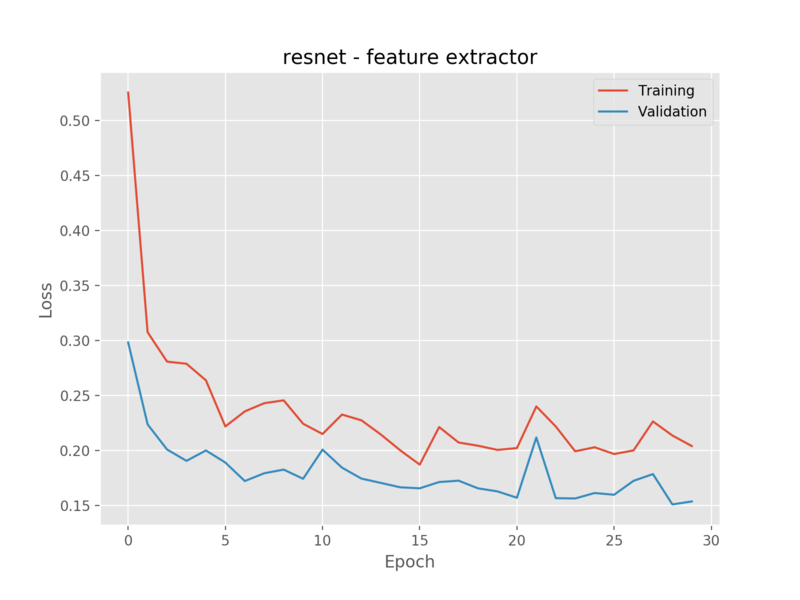
\includegraphics[width=7cm]{b_l_resnet_fe}
  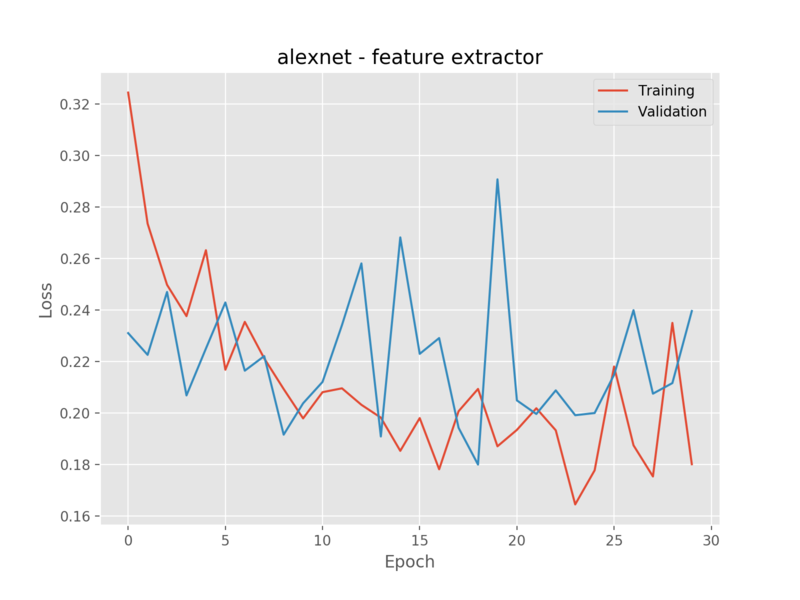
\includegraphics[width=7cm]{b_l_alexnet_fe}
  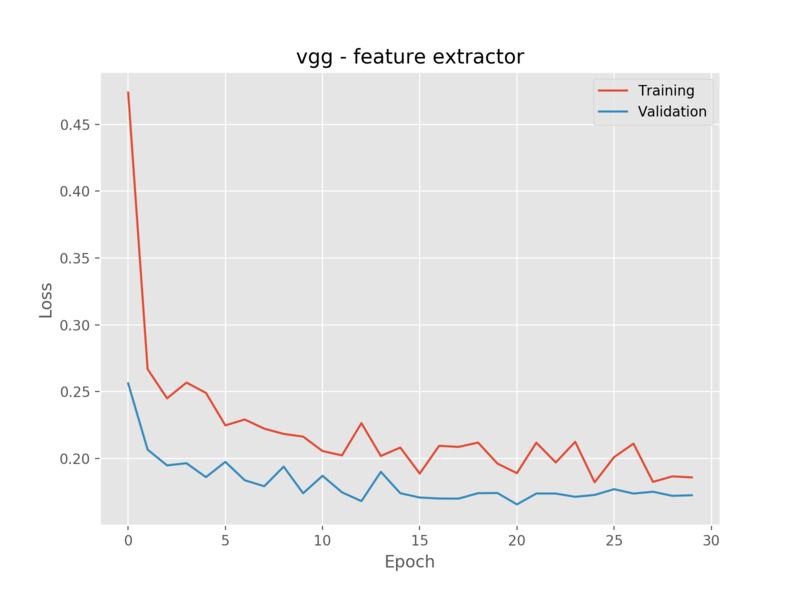
\includegraphics[width=7cm]{b_l_vgg_fe}
  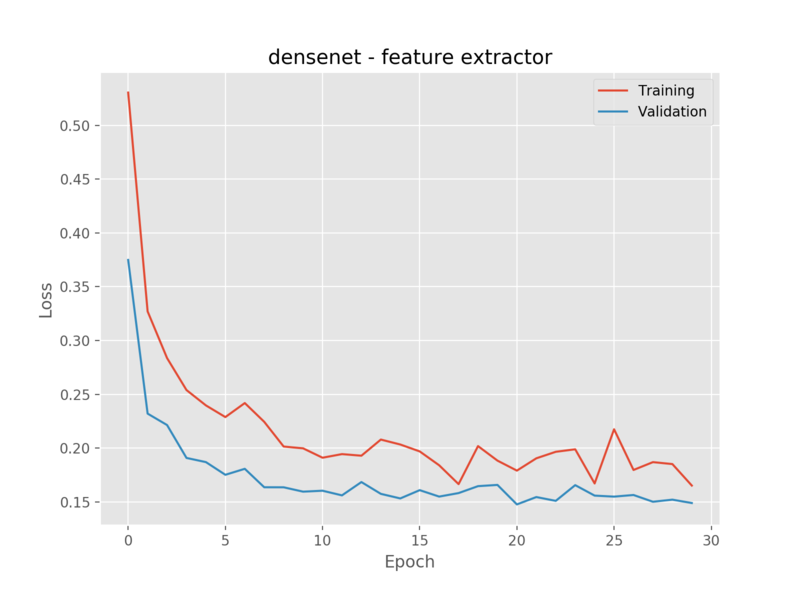
\includegraphics[width=7cm]{b_l_densenet_fe}
  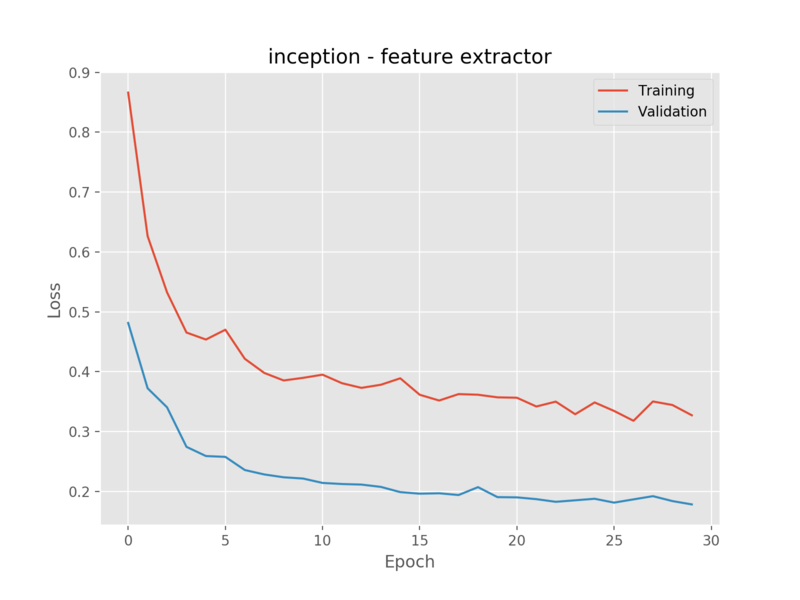
\includegraphics[width=7cm]{b_l_inception_fe}
  \caption{Kostnaden vid varje epoch för balkonger med feature extraction}
  \label{fig:b_l_1}
\end{figure}
\begin{figure}[h]
  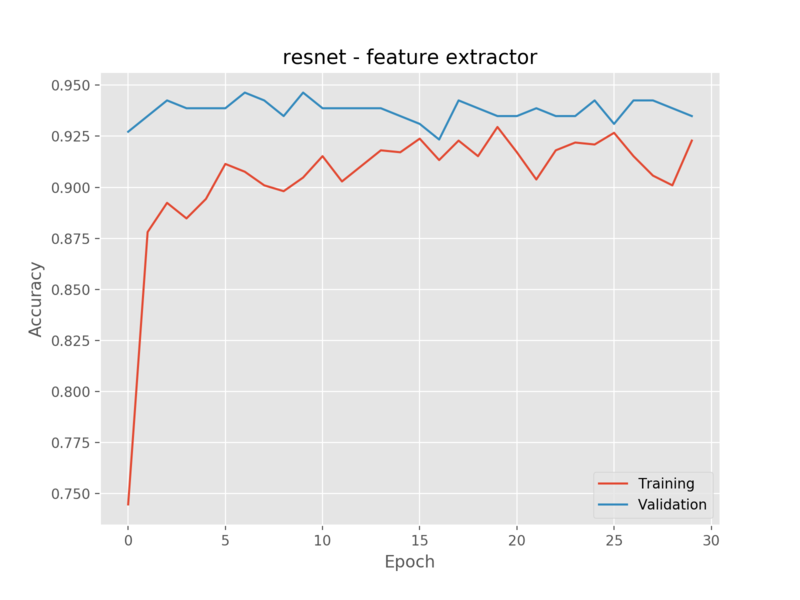
\includegraphics[width=7cm]{b_a_resnet_fe}
  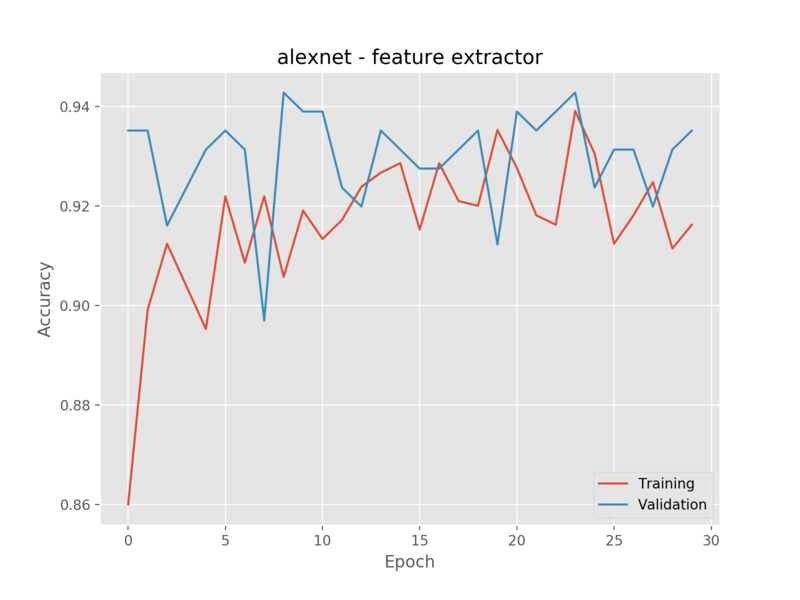
\includegraphics[width=7cm]{b_a_alexnet_fe}
  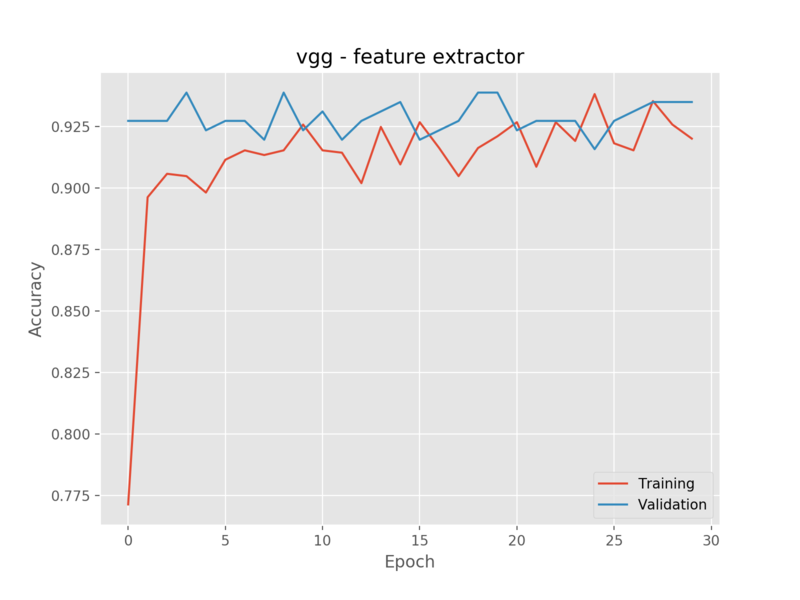
\includegraphics[width=7cm]{b_a_vgg_fe}
  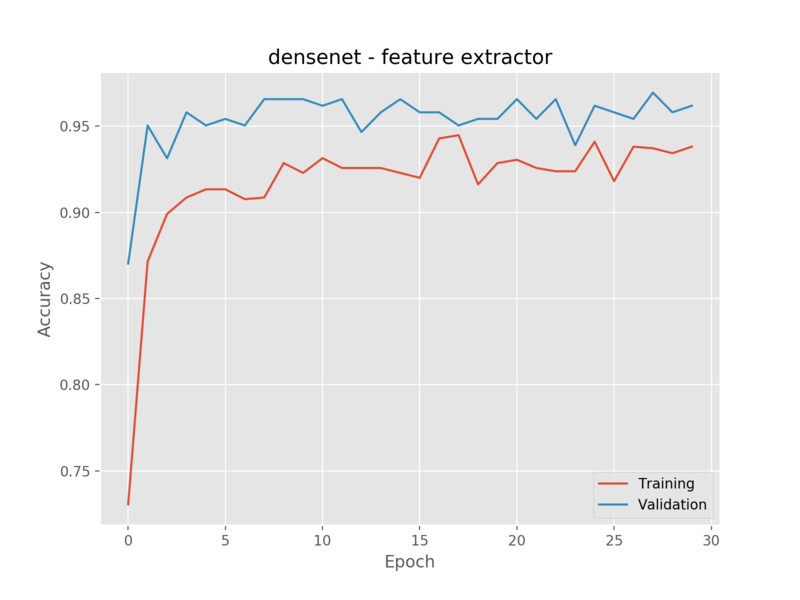
\includegraphics[width=7cm]{b_a_densenet_fe}
  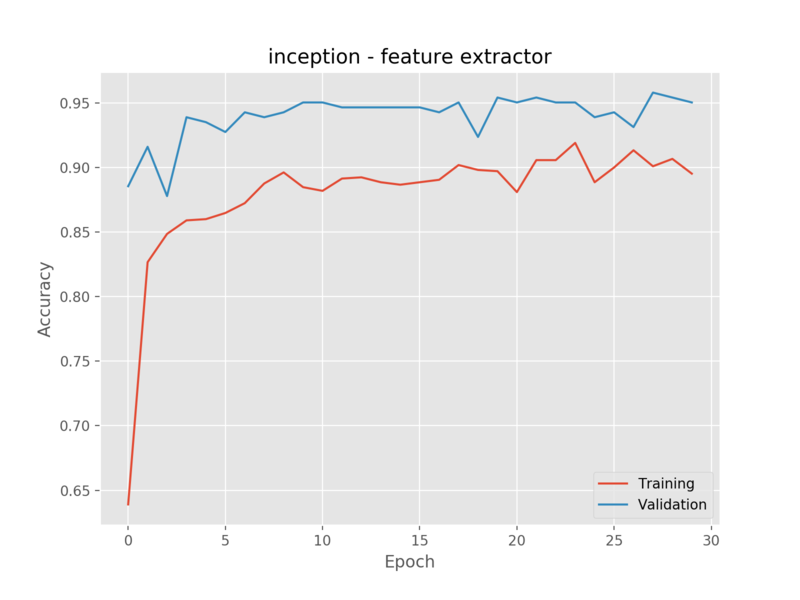
\includegraphics[width=7cm]{b_a_inception_fe}
  \caption{Träffsäkerhet för balkonger med feature extraction}
  \label{fig:b_a_1}
\end{figure}

\subsection{Finetuning}
Vi kan se hur kostnadsfunktionen såg ut för varje epoch i figur \ref{fig:b_l_2} och hur träffsäkerheten var vid finetuning i figur \ref{fig:b_a_2}

\begin{table}
  \centering
  \begin{tabular}{|l|r|r|}
    Modell & Tid & Max. noggrannhet \\ 
    \hline
    Resnet       & 06m 06s & 96.56 \\
    Alexnet      & 03m 37s & 95.41 \\
    VGG-11       & 15m 55s & 97.32 \\
    Densenet     & 13m 55s & 97.70 \\
    Inception V3 & 21m 54s & 98.09 \\
  \end{tabular}
  \caption{Sammanställning av finetuning för balkonger}
\end{table}

\begin{figure}[h]
  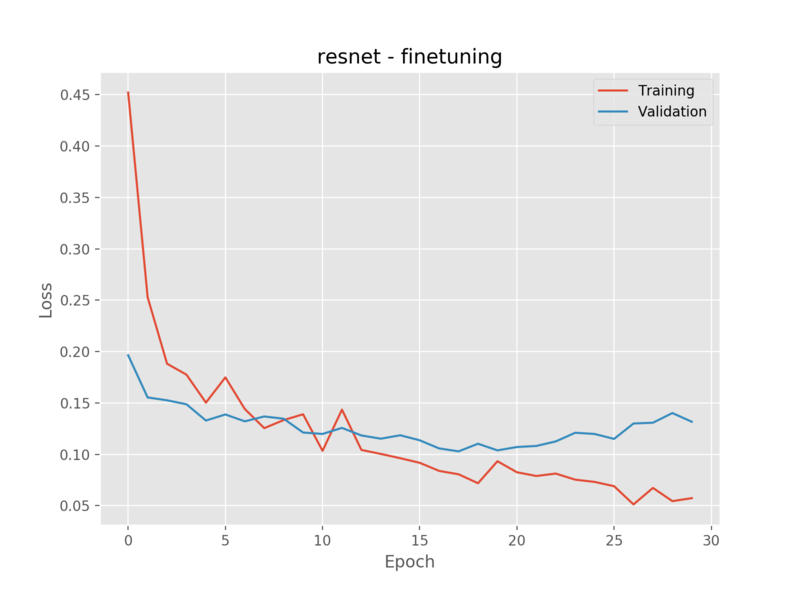
\includegraphics[width=7cm]{b_l_resnet_fine}
  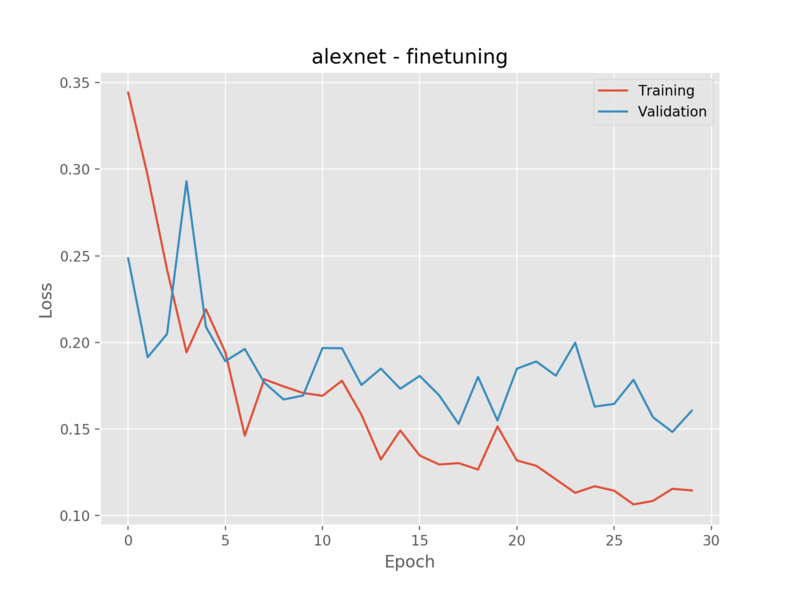
\includegraphics[width=7cm]{b_l_alexnet_fine}
  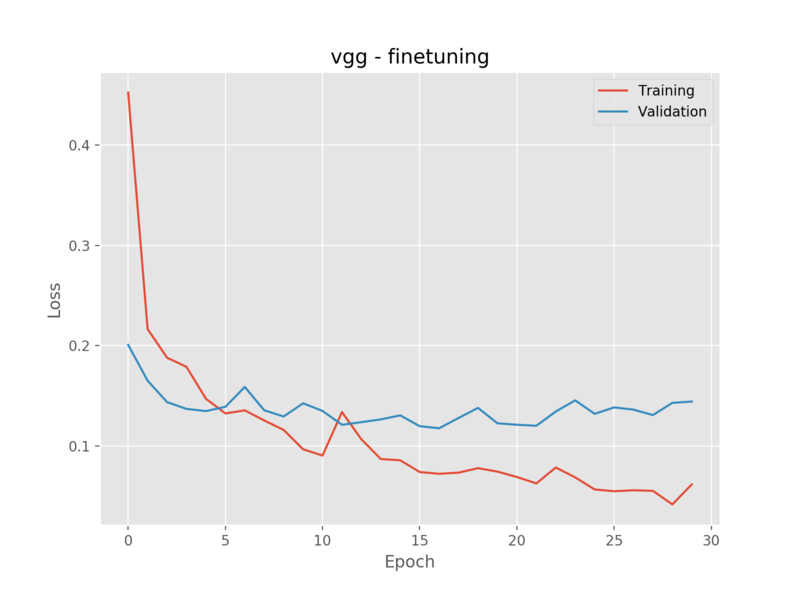
\includegraphics[width=7cm]{b_l_vgg_fine}
  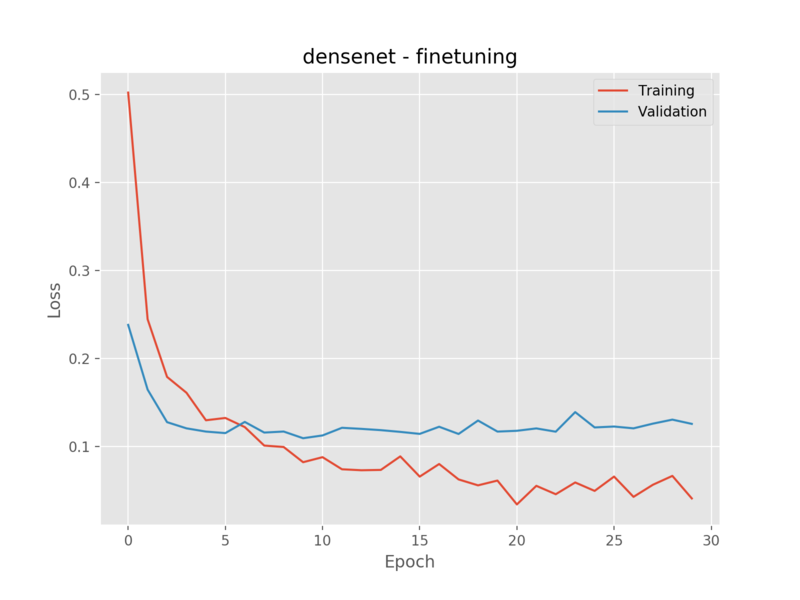
\includegraphics[width=7cm]{b_l_densenet_fine}
  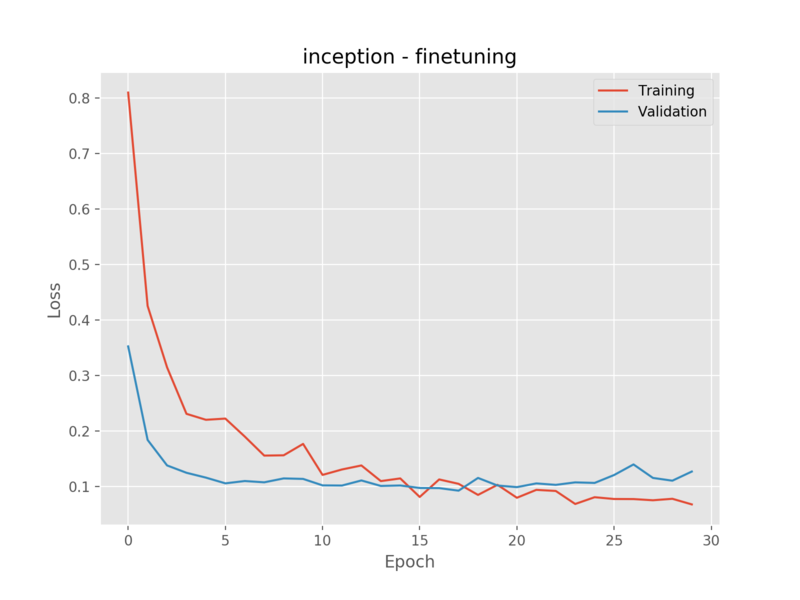
\includegraphics[width=7cm]{b_l_inception_fine}
  \caption{Kostnaden vid varje epoch för balkonger med finetuning}
  \label{fig:b_l_2}
\end{figure}
\begin{figure}[h]
  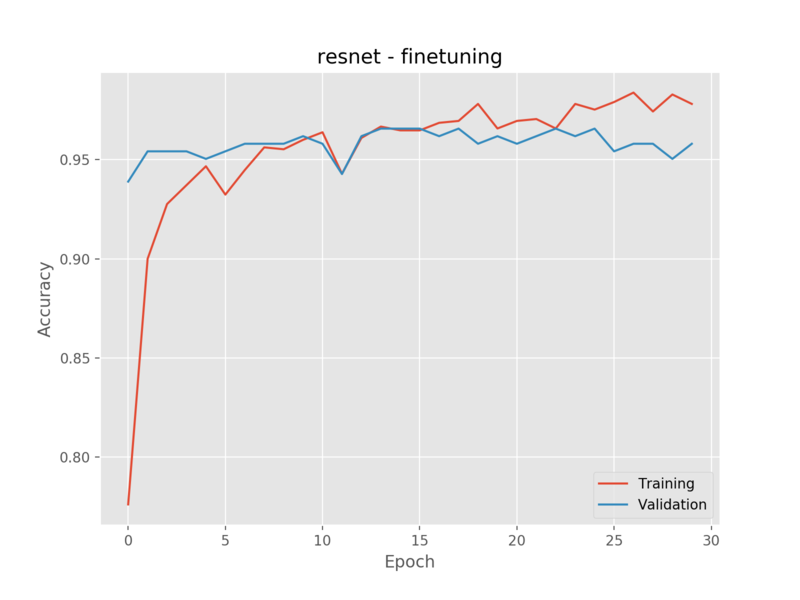
\includegraphics[width=7cm]{b_a_resnet_fine}
  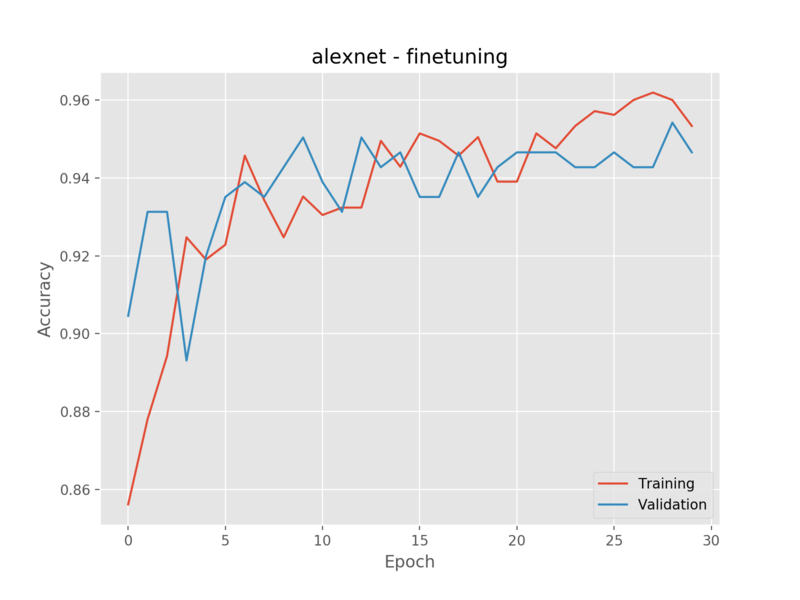
\includegraphics[width=7cm]{b_a_alexnet_fine}
  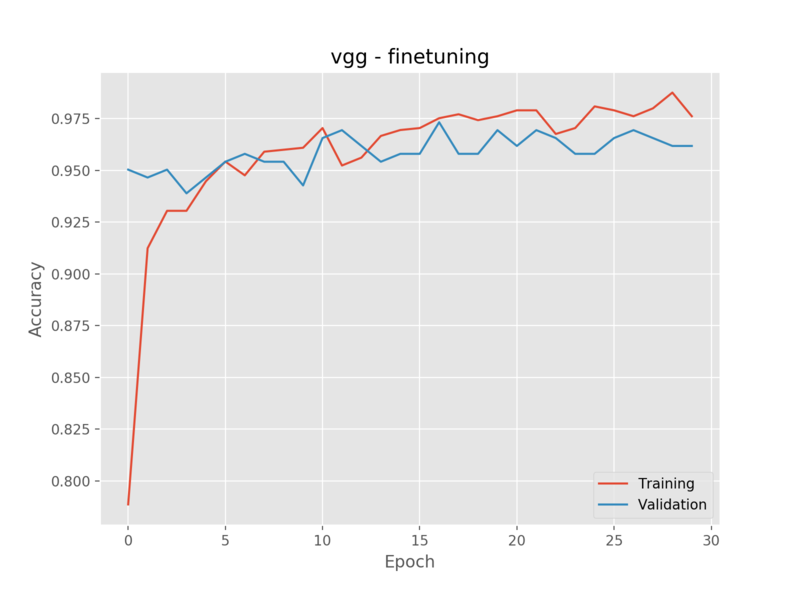
\includegraphics[width=7cm]{b_a_vgg_fine}
  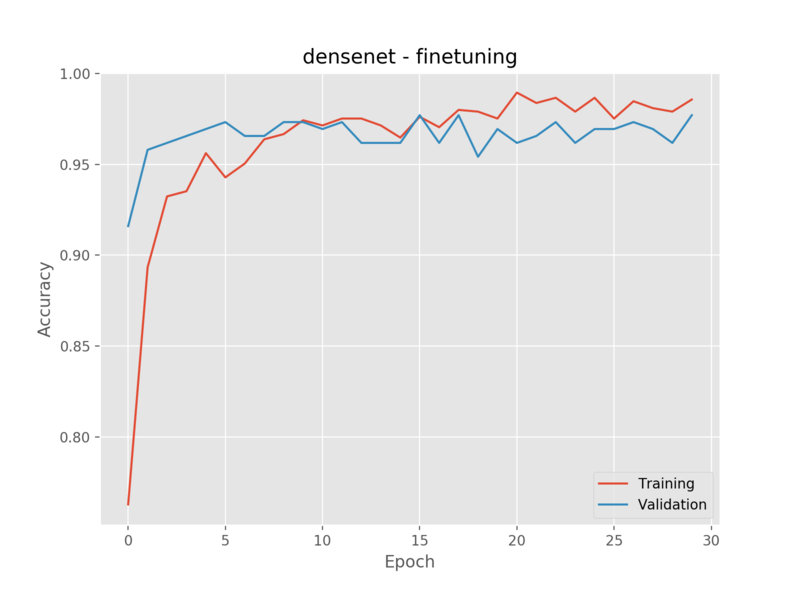
\includegraphics[width=7cm]{b_a_densenet_fine}
  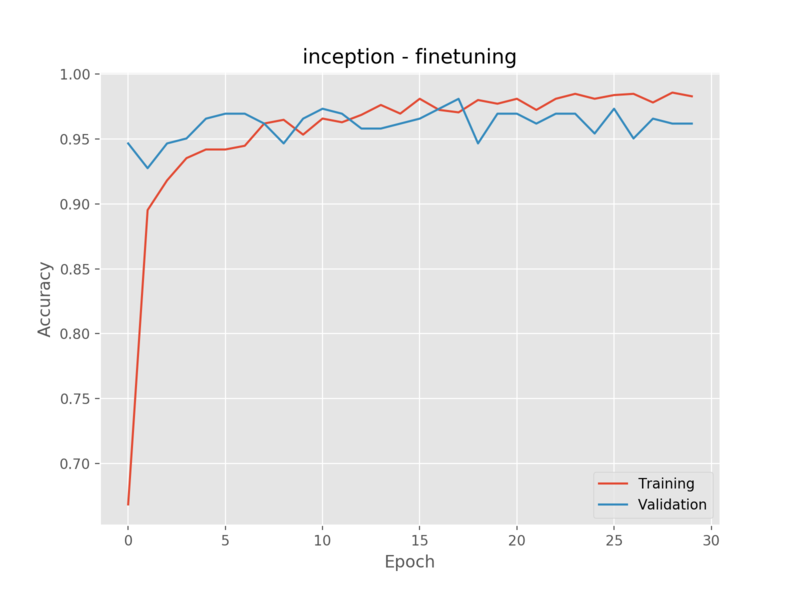
\includegraphics[width=7cm]{b_a_inception_fine}
  \caption{Träffsäkerhet för balkonger med finetuning}
  \label{fig:b_a_2}
\end{figure}

\section{Eldstäder}

\subsection{Feature extraction}
Vi kan se kostnaden för båda tränings och valideringsdatan i figur \ref{fig:f_l_1} för varje epoch. Vi kan även se i figur \ref{fig:f_a_1} hur träffsäkerheten för de olika modeller var på eldstäder.

\begin{table}
  \centering
  \begin{tabular}{|l|r|r|}
    Modell & Tid & Max. noggrannhet \\ 
    \hline
    Resnet       & 02m 06s & 80.50 \\
    Alexnet      & 01m 55s & 80.50 \\
    VGG-11       & 03m 45s & 77.35 \\
    Densenet     & 03m 35s & 73.58 \\
    Inception V3 & 05m 15s & 79.24 \\
  \end{tabular}
  \caption{Sammanställning av feature extraction för eldstäder}
\end{table}

\begin{figure}[h]
  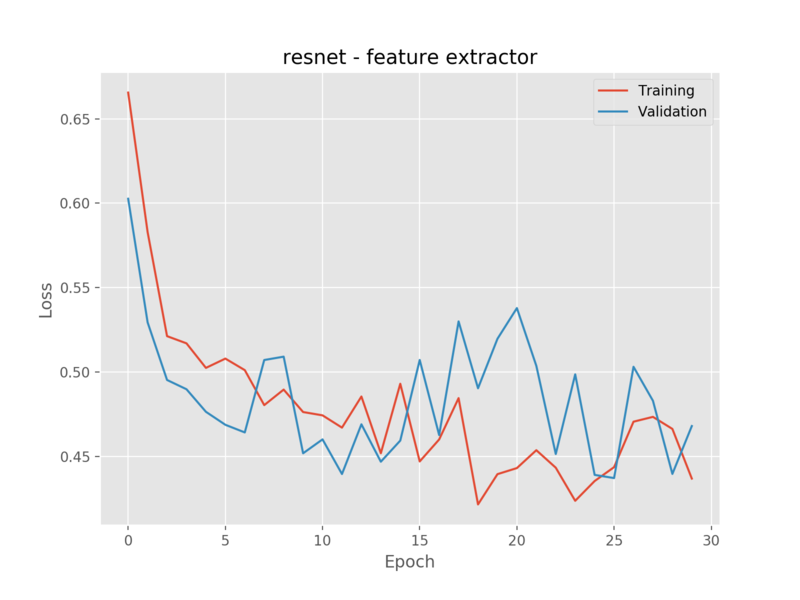
\includegraphics[width=7cm]{f_l_resnet_fe}
  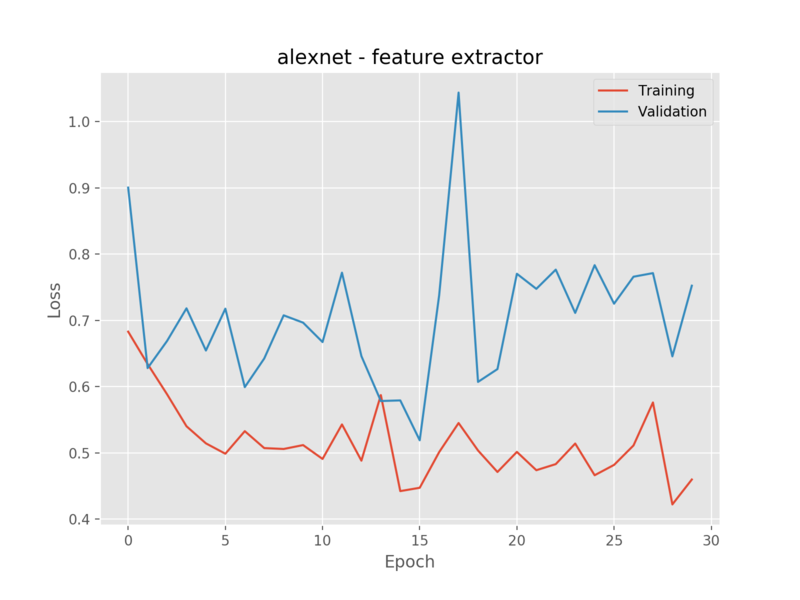
\includegraphics[width=7cm]{f_l_alexnet_fe}
  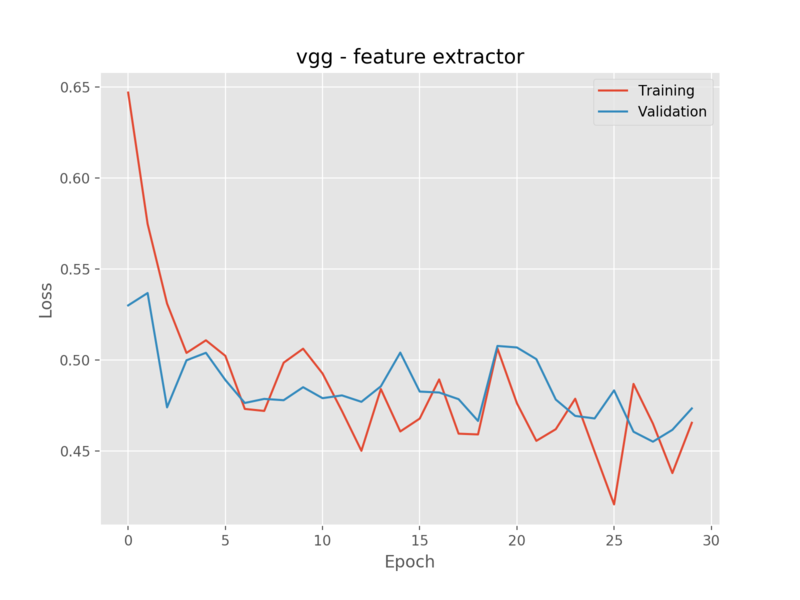
\includegraphics[width=7cm]{f_l_vgg_fe}
  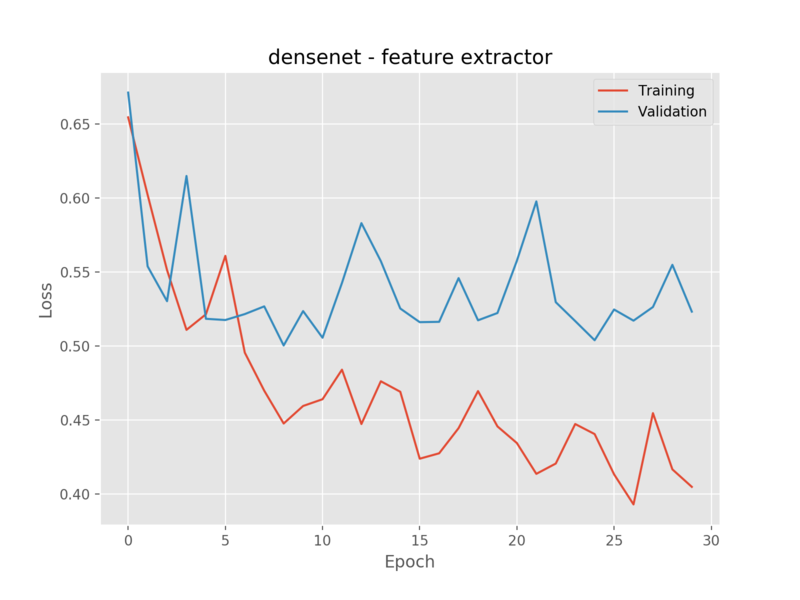
\includegraphics[width=7cm]{f_l_densenet_fe}
  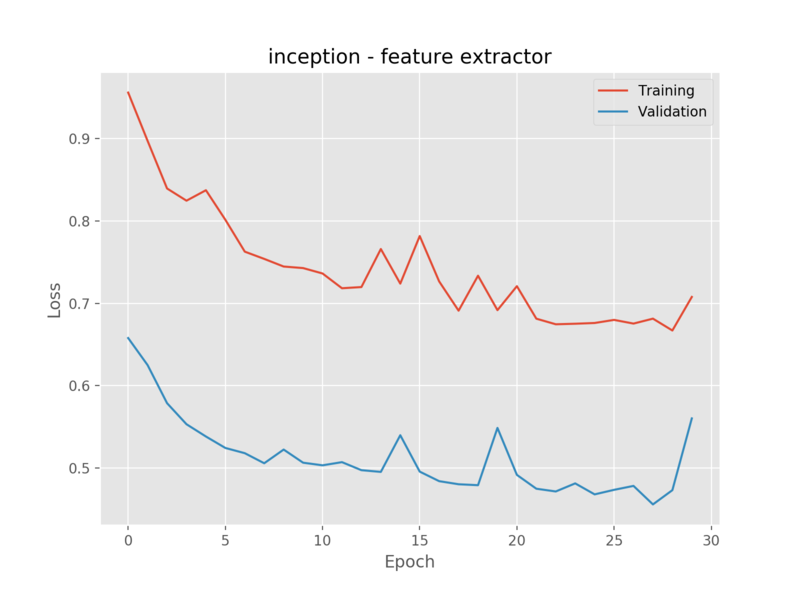
\includegraphics[width=7cm]{f_l_inception_fe}
  \caption{Kostnaden vid varje epoch för eldstäder med feature extraction}
  \label{fig:f_l_1}
\end{figure}
\begin{figure}[h]
  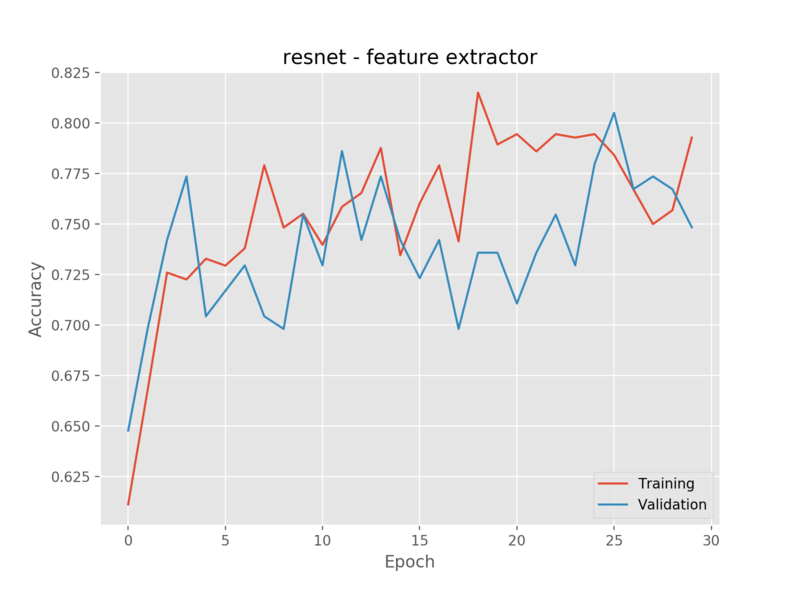
\includegraphics[width=7cm]{f_a_resnet_fe}
  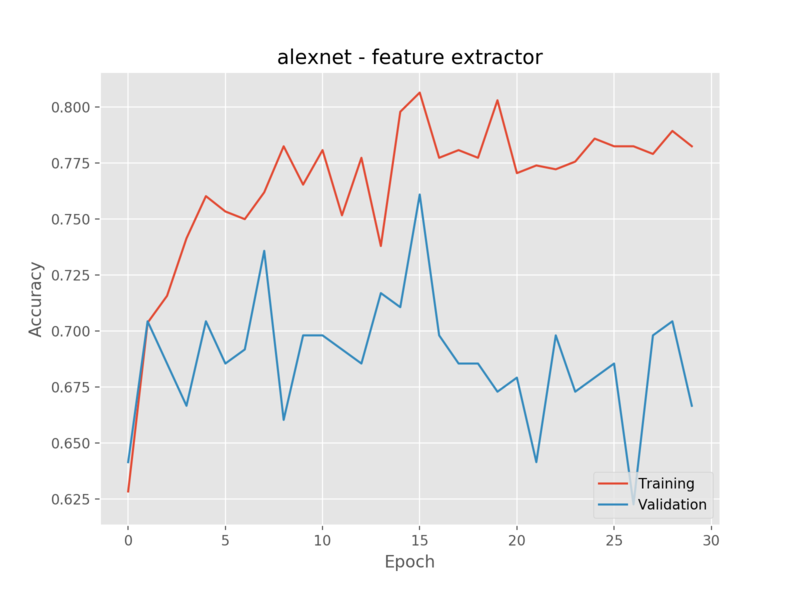
\includegraphics[width=7cm]{f_a_alexnet_fe}
  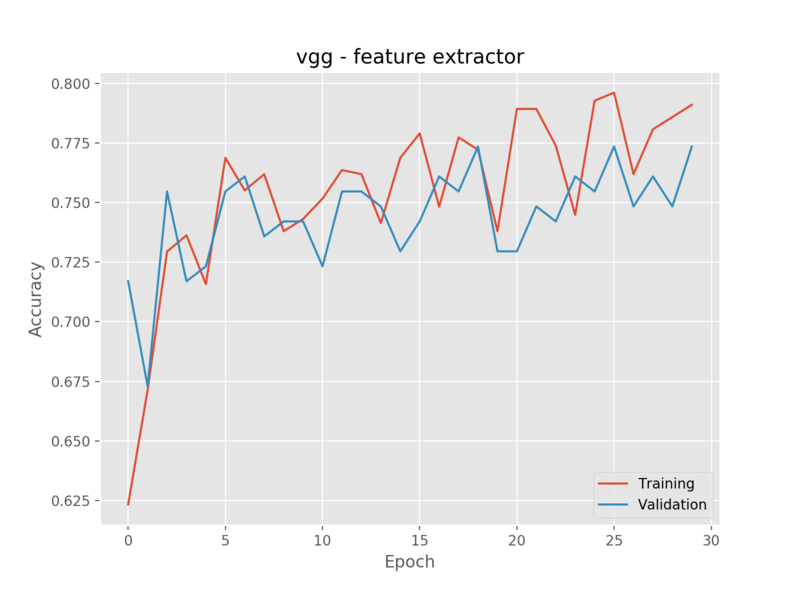
\includegraphics[width=7cm]{f_a_vgg_fe}
  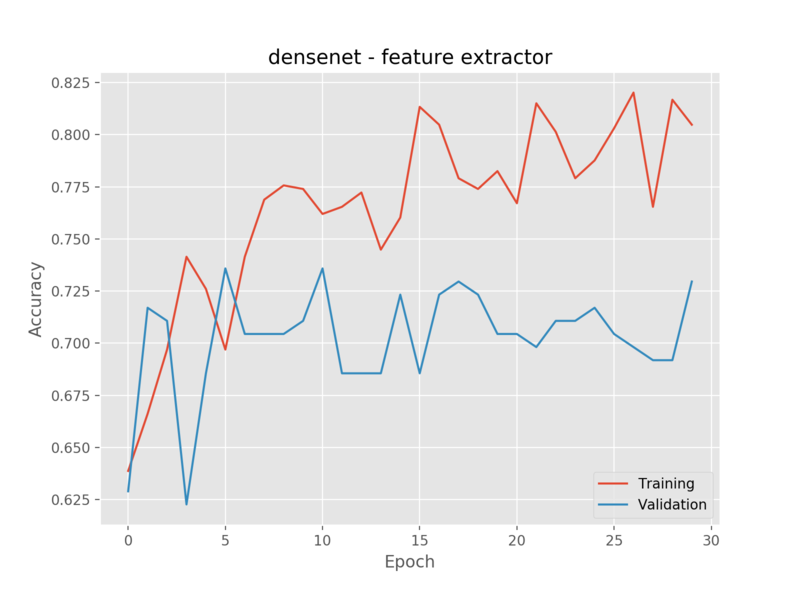
\includegraphics[width=7cm]{f_a_densenet_fe}
  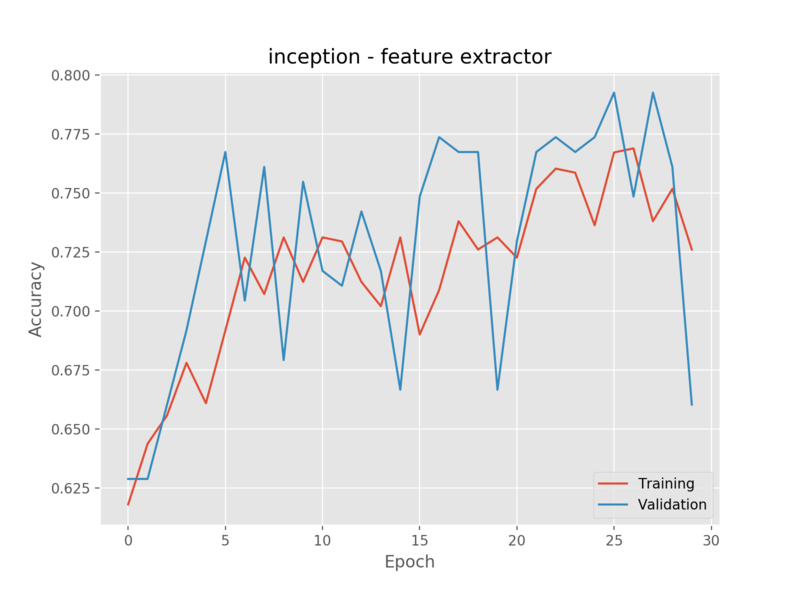
\includegraphics[width=7cm]{f_a_inception_fe}
  \caption{Träffsäkerhet för eldstäder med feature extraction}
  \label{fig:f_a_1}
\end{figure}

\subsection{Finetuning}
Vi kan se hur kostnadsfunktionen såg ut för varje epoch i figur \ref{fig:f_l_2} och hur träffsäkerheten var vid finetuning i figur \ref{fig:f_a_2}

\begin{table}
  \centering
  \begin{tabular}{|l|r|r|}
    Modell & Tid & Max. noggrannhet \\ 
    \hline
    Resnet       & 03m 31s & 79.24 \\
    Alexnet      & 02m 08s & 77.35 \\
    VGG-11       & 08m 56s & 81.13 \\
    Densenet     & 07m 55s & 85.53 \\
    Inception V3 & 12m 54s & 83.64 \\
  \end{tabular}
  \caption{Sammanställning av finetuning för eldstäder}
\end{table}

\begin{figure}[h]
  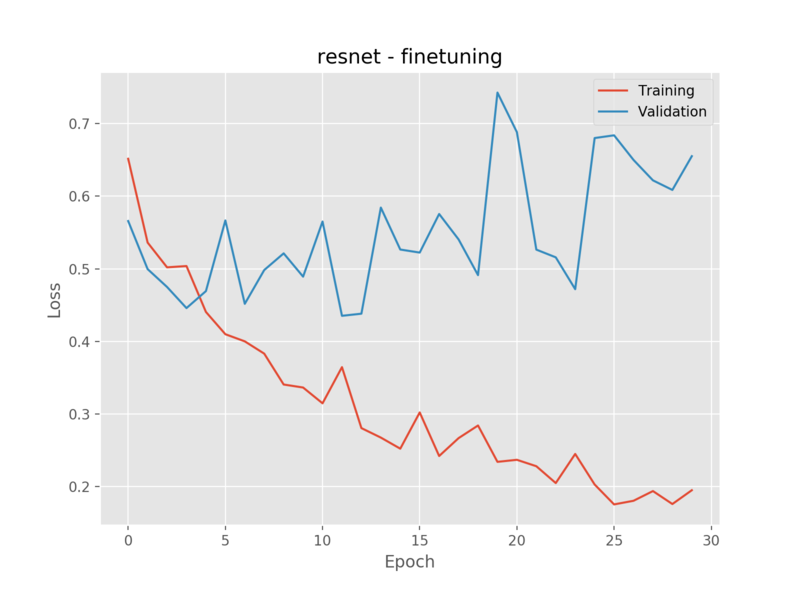
\includegraphics[width=7cm]{f_l_resnet_fine}
  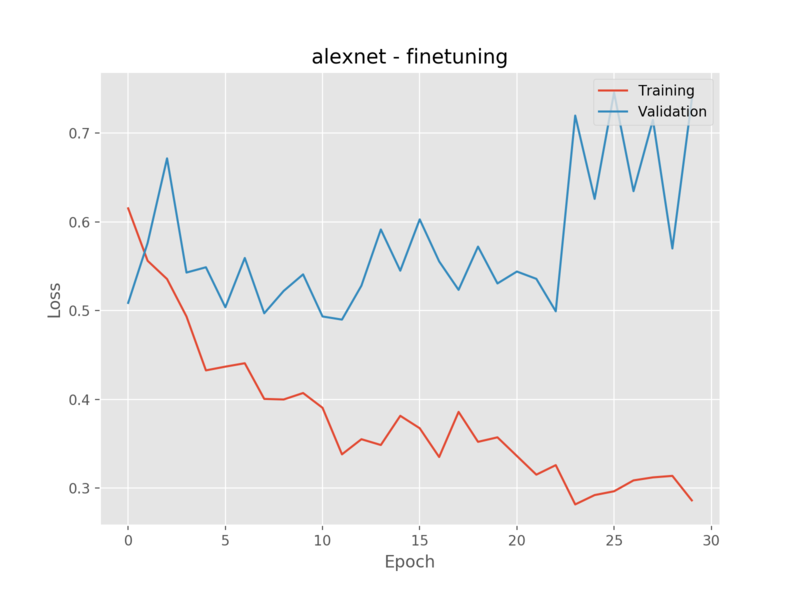
\includegraphics[width=7cm]{f_l_alexnet_fine}
  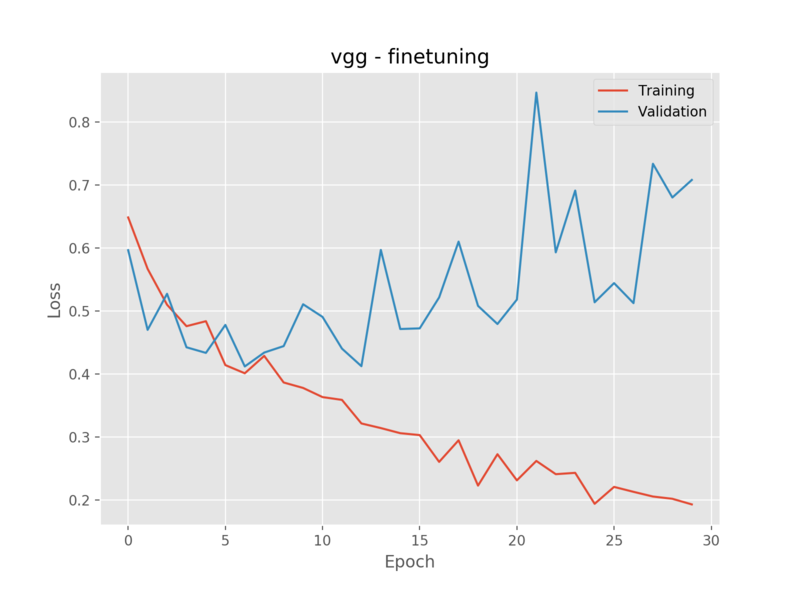
\includegraphics[width=7cm]{f_l_vgg_fine}
  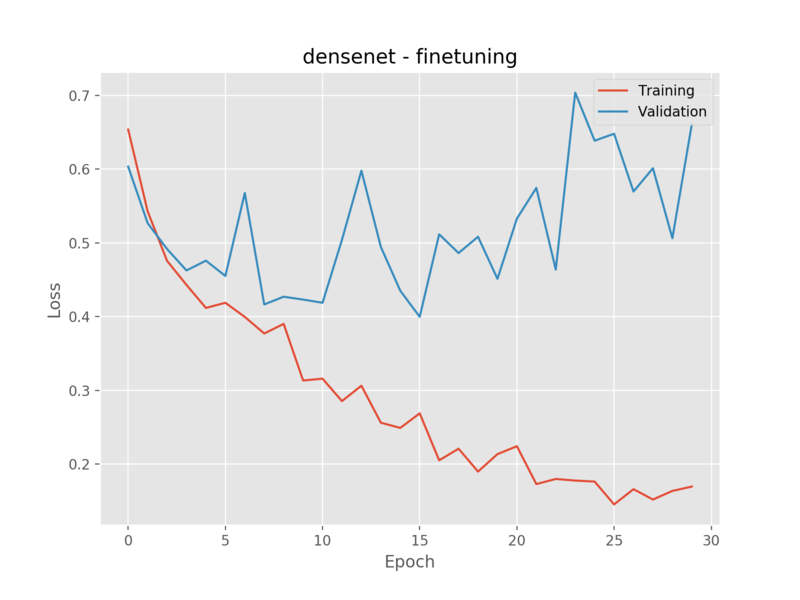
\includegraphics[width=7cm]{f_l_densenet_fine}
  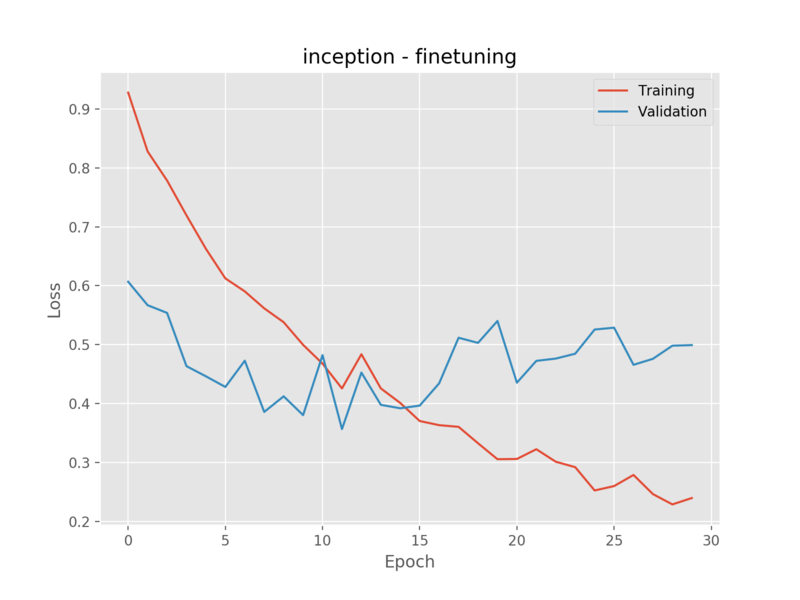
\includegraphics[width=7cm]{f_l_inception_fine}
  \caption{Kostnaden vid varje epoch för eldstäder med finetuning}
  \label{fig:f_l_2}
\end{figure}
\begin{figure}[h]
  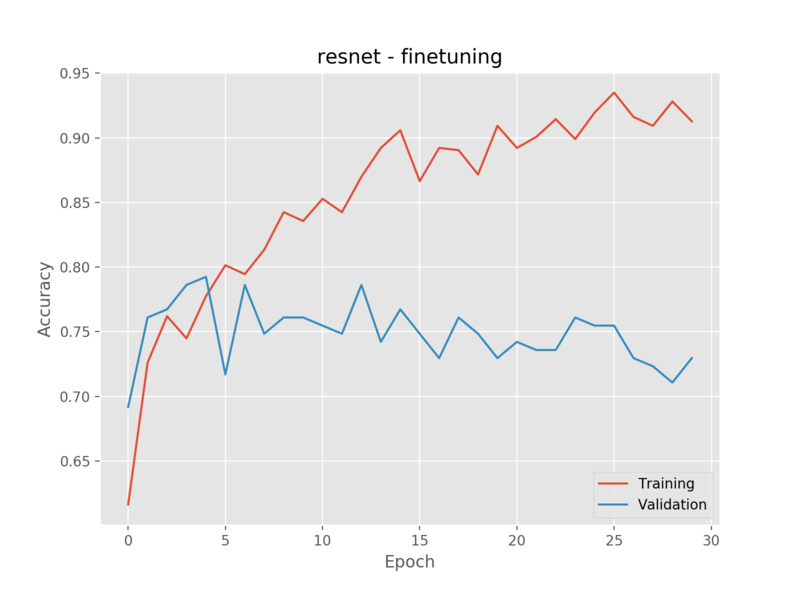
\includegraphics[width=7cm]{f_a_resnet_fine}
  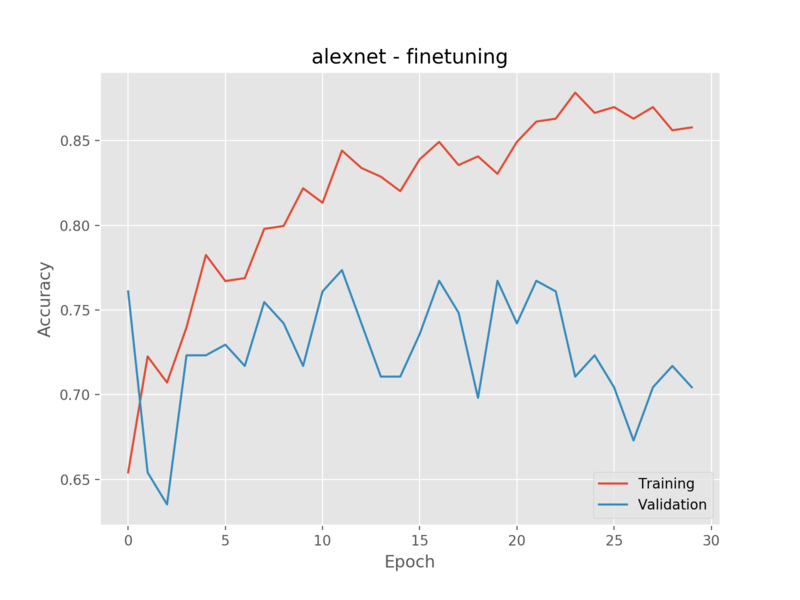
\includegraphics[width=7cm]{f_a_alexnet_fine}
  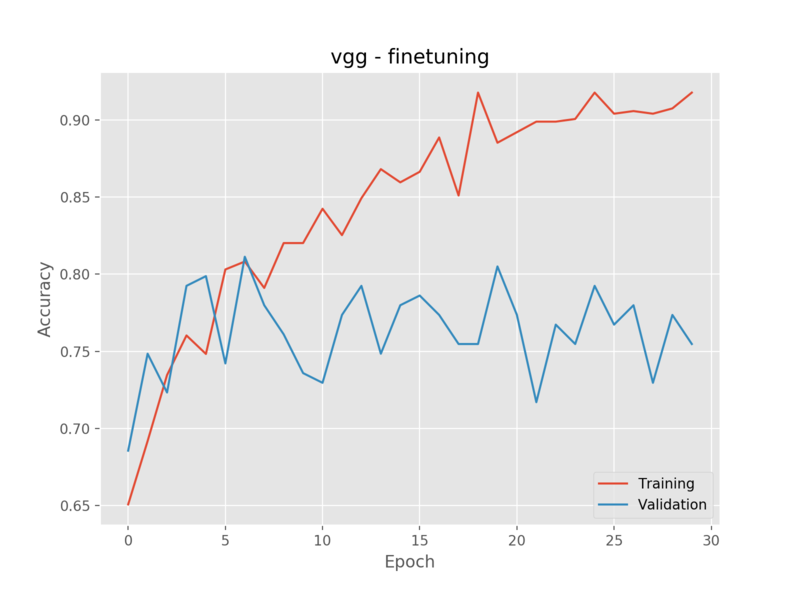
\includegraphics[width=7cm]{f_a_vgg_fine}
  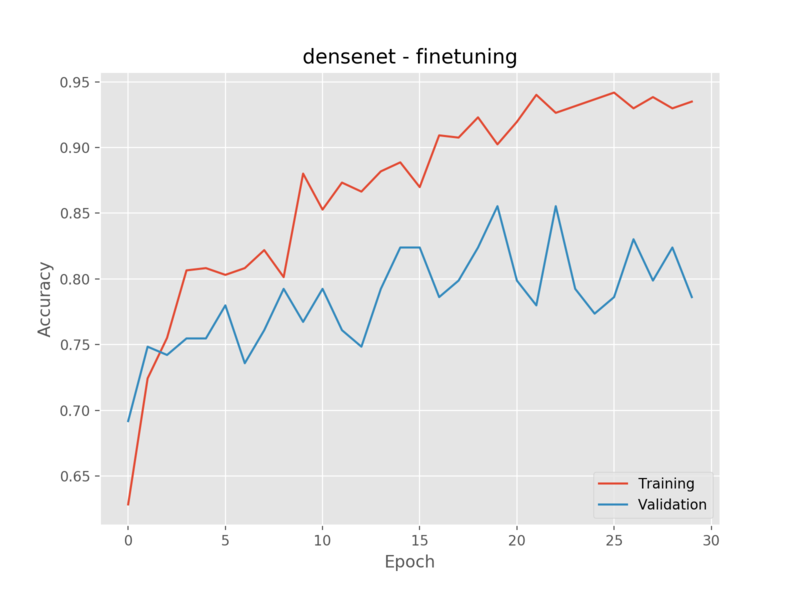
\includegraphics[width=7cm]{f_a_densenet_fine}
  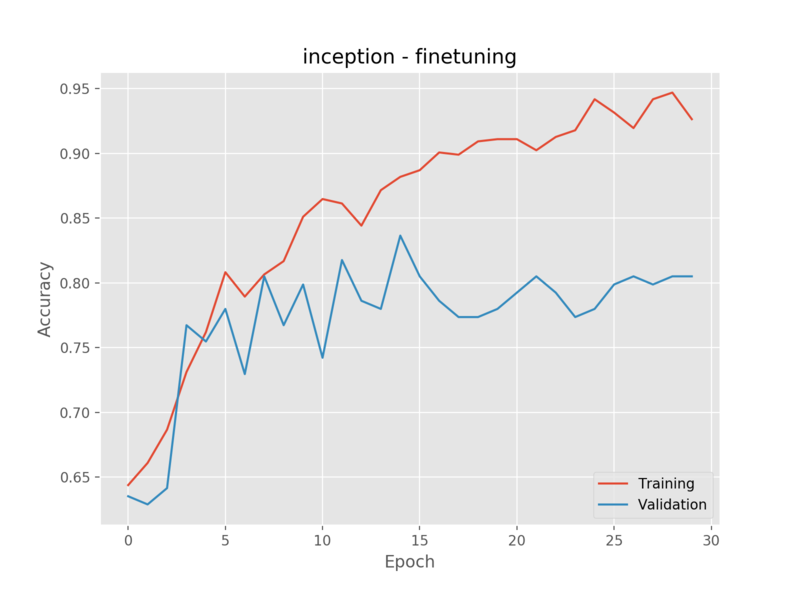
\includegraphics[width=7cm]{f_a_inception_fine}
  \caption{Träffsäkerhet för eldstäder med finetuning}
  \label{fig:f_a_2}
\end{figure}

\section{Rum}

\subsection{Feature extraction}
Vi kan se kostnaden för båda tränings och valideringsdatan i figur \ref{fig:r_l_1} för varje epoch. Vi kan även se i figur \ref{fig:r_a_1} hur träffsäkerheten för de olika modeller var på rum.

\begin{table}
  \centering
  \begin{tabular}{|l|r|r|}
    Modell & Tid & Max. noggrannhet \\ 
    \hline
    Resnet       & 02m 33s & 93.75 \\
    Alexnet      & 02m 18s & 93.22 \\
    VGG-11       & 04m 31s & 93.75 \\
    Densenet     & 04m 20s & 96.87 \\
    inception V3 & 06m 28s & 93.75 \\
  \end{tabular}
  \caption{Sammanställning av feature extraction för rum}
\end{table}

\begin{figure}[h]
  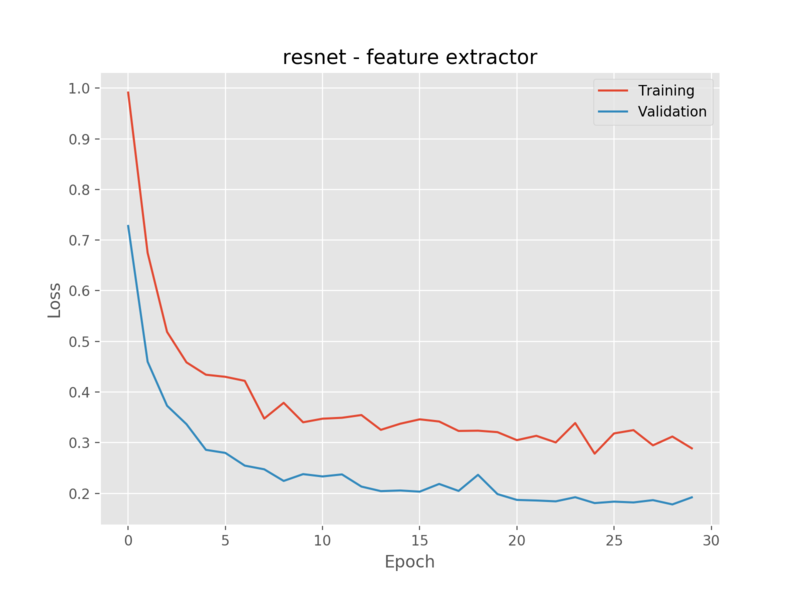
\includegraphics[width=7cm]{r_l_resnet_fe}
  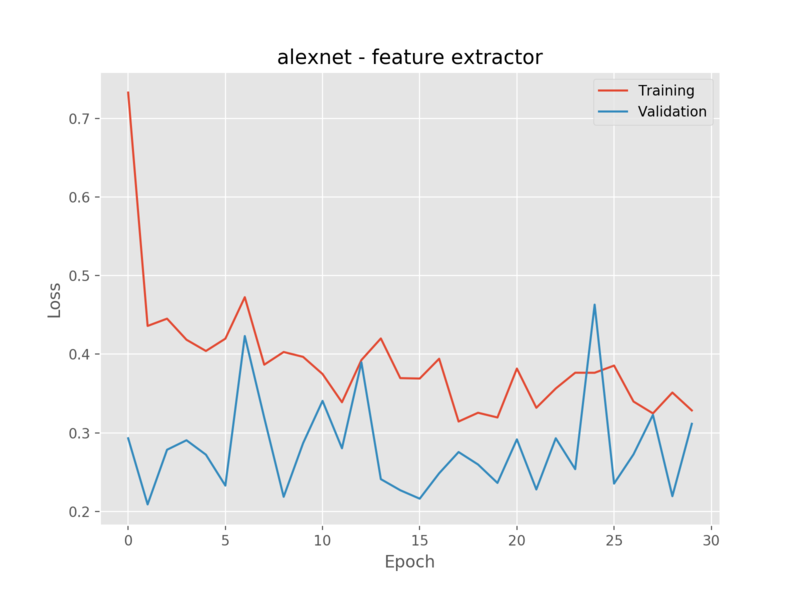
\includegraphics[width=7cm]{r_l_alexnet_fe}
  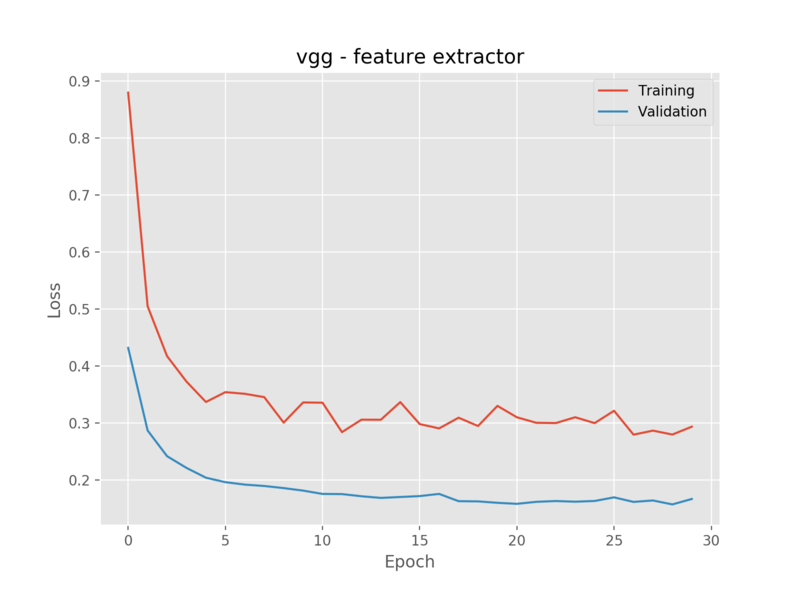
\includegraphics[width=7cm]{r_l_vgg_fe}
  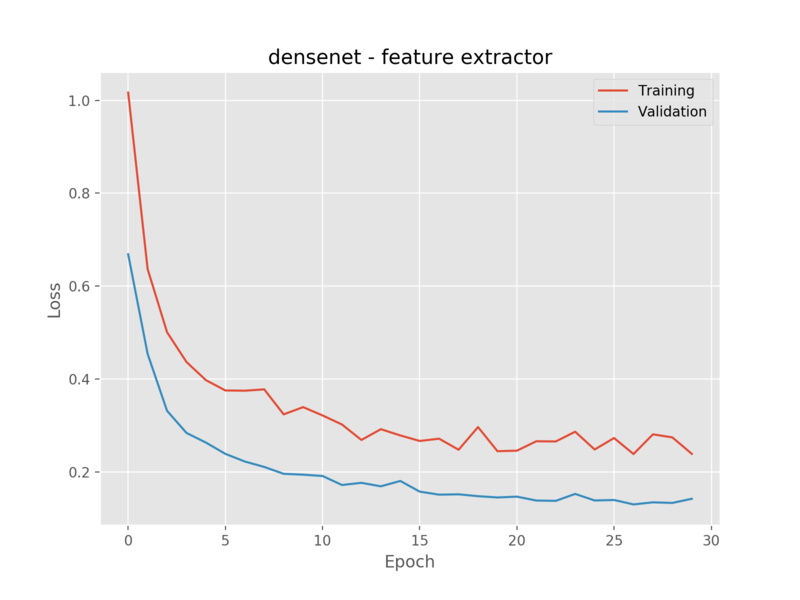
\includegraphics[width=7cm]{r_l_densenet_fe}
  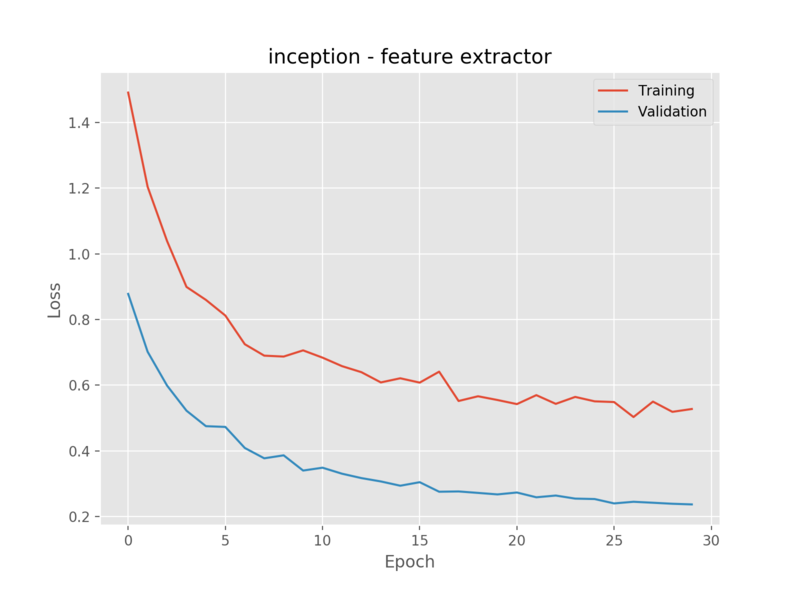
\includegraphics[width=7cm]{r_l_inception_fe}
  \caption{Kostnaden vid varje epoch för rum med feature extraction}
  \label{fig:r_l_1}
\end{figure}
\begin{figure}[h]
  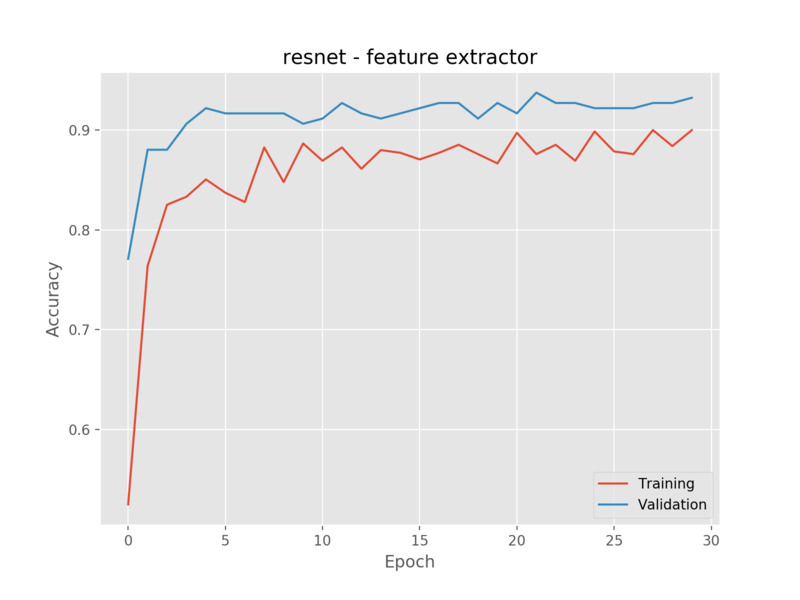
\includegraphics[width=7cm]{r_a_resnet_fe}
  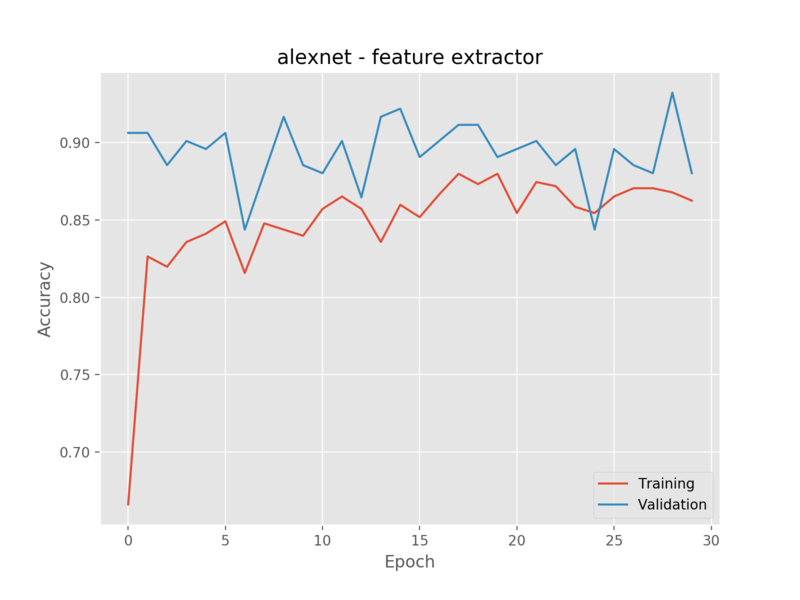
\includegraphics[width=7cm]{r_a_alexnet_fe}
  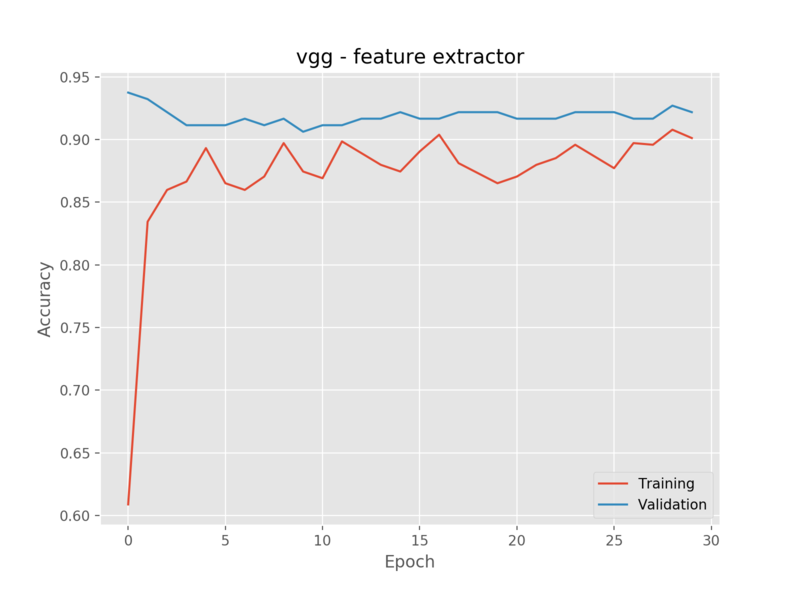
\includegraphics[width=7cm]{r_a_vgg_fe}
  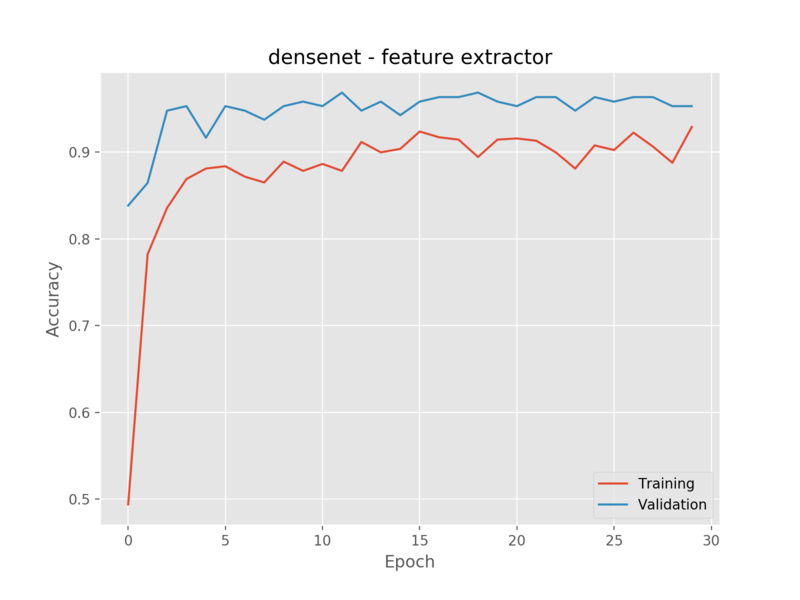
\includegraphics[width=7cm]{r_a_densenet_fe}
  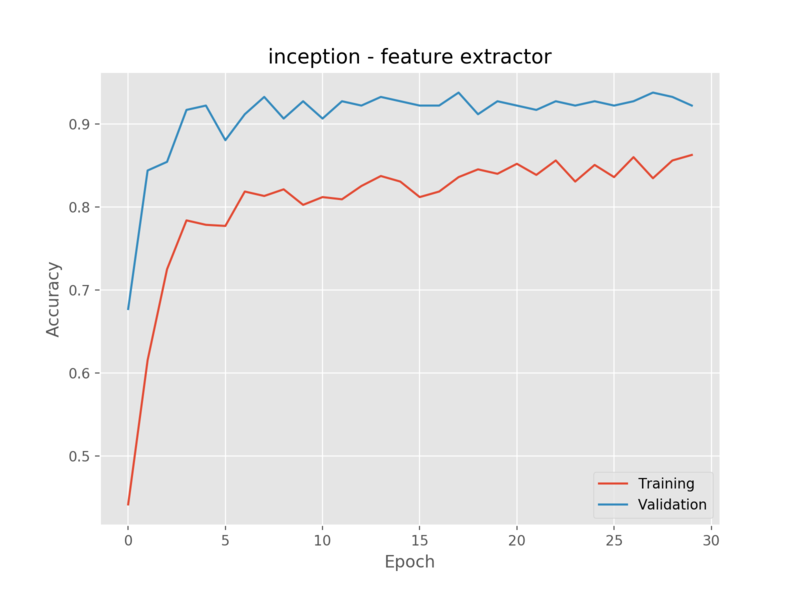
\includegraphics[width=7cm]{r_a_inception_fe}
  \caption{Träffsäkerhet för rum med feature extraction}
  \label{fig:r_a_1}
\end{figure}

\subsection{Finetuning}
Vi kan se hur kostnadsfunktionen såg ut för varje epoch i figur \ref{fig:r_l_2} och hur träffsäkerheten var vid finetuning i figur \ref{fig:r_a_2}

\begin{table}
  \centering
  \begin{tabular}{|l|r|r|}
    Modell & Tid & Max. noggrannhet \\ 
    \hline
    Resnet       & 04m 16s & 96.35 \\
    Alexnet      & 02m 34s & 94.79 \\
    VGG-11       & 11m 02s & 97.91 \\
    Densenet     & 09m 53s & 97.91 \\
    Inception V3 & 16m 10s & 97.39 \\
  \end{tabular}
  \caption{Sammanställning av finetuning för rum}
\end{table}

\begin{figure}[h]
  \includegraphics[width=7cm]{r_l_resnet_fine}
  \includegraphics[width=7cm]{r_l_alexnet_fine}
  \includegraphics[width=7cm]{r_l_vgg_fine}
  \includegraphics[width=7cm]{r_l_densenet_fine}
  \includegraphics[width=7cm]{r_l_inception_fine}
  \caption{Kostnaden vid varje epoch för rum med finetuning}
  \label{fig:r_l_2}
\end{figure}
\begin{figure}[h]
  \includegraphics[width=7cm]{r_a_resnet_fine}
  \includegraphics[width=7cm]{r_a_alexnet_fine}
  \includegraphics[width=7cm]{r_a_vgg_fine}
  \includegraphics[width=7cm]{r_a_densenet_fine}
  \includegraphics[width=7cm]{r_a_inception_fine}
  \caption{Träffsäkerhet för rum med finetuning}
  \label{fig:r_a_2}
\end{figure}

\chapter{Diskussion}
Diskutera resultatet och hur olika delar kan ha påverkat eller påverkade. Diskutera eventuell framtida forskning. Begränsningar med resultatet. Etiska aspekter. Hållbarhet.

\section{Fortsatt forskning}
Vid värdering så är det också intressant att få ut attribut, så kan man räkna med det i värderingskalkylen.

\chapter{Slutsats}  
Slutsats av vad vi kom fram till.

\printbibliography[heading=bibintoc]
\appendix
  \chapter{Appendix A}

\tailmatter
\end{document}
